

\chapter{Hydrodynamics - Fundamental Equations}


\section{Levels of theory}

Level 0 to 1:  The separation between particles should be much larger
than de Broglie wavelength, otherwise the particles will experience
quantum interference. 

The de Broglie wavelength is 

\beq
\lambda = \frac{h}{p}
\eeq

\noindent write the momentum in terms of the energy and consider the energy to
be thermal

\beq
p \sqrt{2mE} \sim \sqrt{m kT}
\eeq

\noindent $\lambda$ must be much smaller than the separation between particles,
which is $n^{-1/3}$, where $n$ is the number density. The condition
for the particles to be treated as classical is thus 

\beq
\frac{h n^{1/3}}{\sqrt{m kT}} \ll 1
\eeq


Level 1 to 2: when N becomes too large, then it's impractical to solve
$N\ll 1$ equations. Define then the distribution function $f$ for the
particle number density in phase space. This is only possible when the
system is either collisionless or if binary collisions are the only
interaction between particles.

Level 2 to 3: Through frequent binary collisions, the system relaxes
to the Maxwell-Boltzmann distribution. This occurs if the mean-free
path is small compared to the length scale of the system. Otherwise, a
distribution function needs to be applied (in this case a continuity
equation still can be used, but the ``fluid'' contains no pressure). 

\classcomm{Do ``show of hands'' for ISM, atmosphere, pp-disk, etc, if
they can be described as fluids.}

\section{Macroscopic view}

We will think of a fluid first in macroscopic terms. Consider a 
{\it fluid element}. A fluid elements is a region over which we can
define local variables, such as density, temperature, etc, see \fig{fig:riogrande}

\begin{figure}
  \begin{center}
    \resizebox{\textwidth}{!}{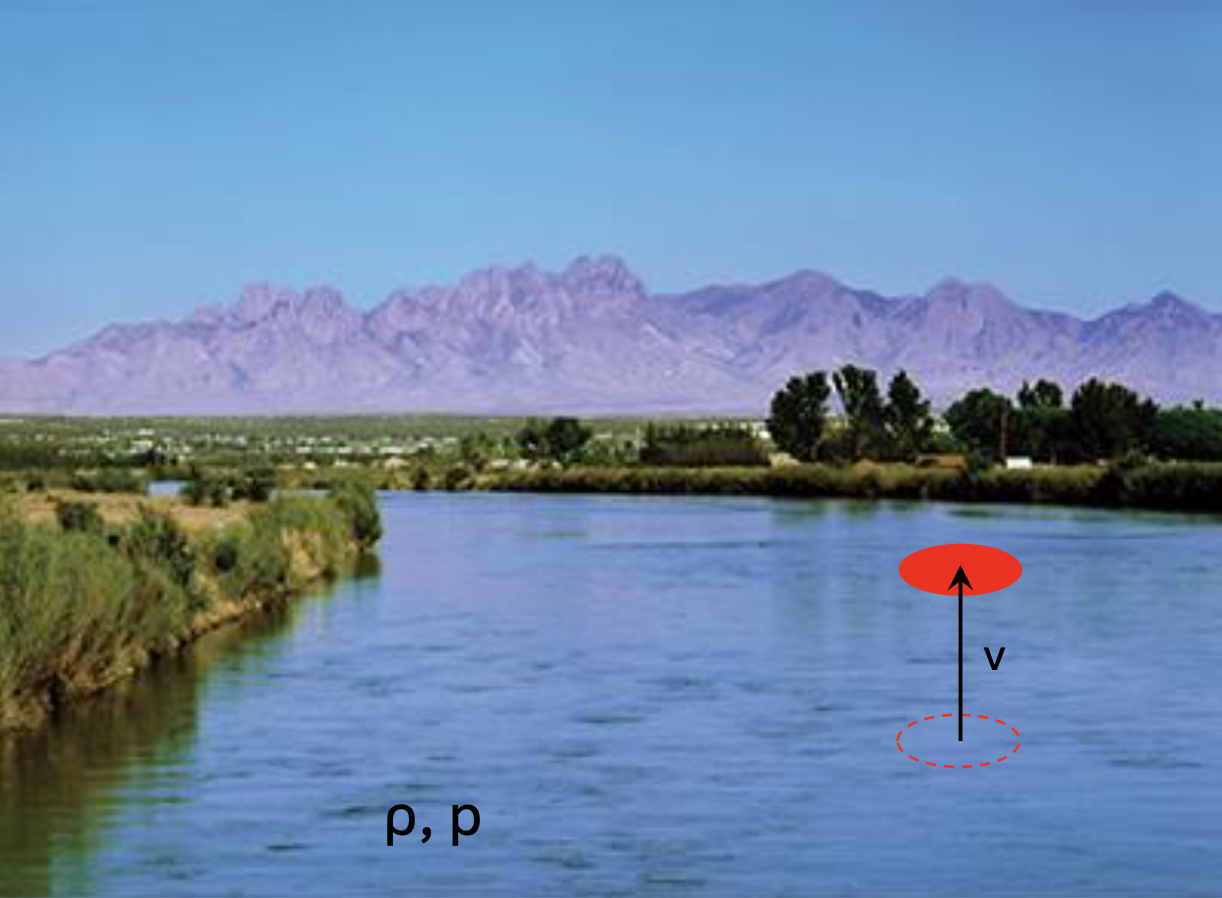
\includegraphics{./figs/riogrande.png}}
  \end{center}
  \caption[]{A fluid element is a region
over which we can define
local variables (density, temperature, etc), and it moves with a bulk velocity, the
mean flow velocity. To be uniform, this patch
must be mall enough that we
can ignore systematic
variations across it for
any variable, large enough to contain
sufficient particles to
ignore fluctuations due
to the finite
number of particles, and much bigger than mean
free path.}
  \label{fig:riogrande}
\end{figure}


The size of this patch (length scale $l_{\rm patch}$ ) is assumed to
be such that it is

\begin{itemize}

\item small enough that we can ignore systematic variations across it for any
variable $q$ we are interested in:

\begin{equation}
l_{\rm patch} \ll \frac{q}{|\grad{q}|}
\end{equation}

That is, the patch is homogeneus and uniform. 

\item large enough to contain sufficient particles to ignore fluctuations due to
the finite number of particles (discreteness noise):

\begin{equation}
nl^3_{\rm patch} \gg 1
\end{equation}


\item In addition, collisional fluids must satisfy: $l_{\rm patch} \gg
  l_{\rm mfp}$ where $l_{\rm mfp}$ is the mean free path of particles

\end{itemize}
  
The mean path is

\begin{equation}
%  l_{\rm mfp} = \frac{1}{\sqrt{2} n pi a^2}
    l_{\rm mfp} \sim \frac{1}{n \sigma}
\end{equation}

\noindent where $\sigma$ is the cross section of particles and $n$ their number
density. The typical molecular cross section is $10^{-15}$ cm$^{2}$.

For air, the number density is $10^{19}$ cm$^{-3}$, implying mean free path
$10^{-4}$ cm. Typical human scales being cm- to km-sized, a fluid
description is valid. 

For a protoplanetary disk, the density is $10^{14}$ cm$^{-3}$, so the mean
free path is $10$ cm. The scale height being AUs, and typical scales
10s of AUs, the fluid description is appropriate. 

For the ISM, the density is 10 cm$^{-3}$, so the mean
free path is $10^{14}$ cm (about 10AU). The scale height being
hundreds of parsecs, and typical scales 10s of parsecs, the fluid
description is appropriate.

When does it break down? Gas in debris disks, for instance. Or
cometary tails.

For gas in debris disks, the density is 100 $^{-3}$ at 100 au, so a
mean free path of about 0.1 AU is estimated. With structure of the
order of au, this is barely within the applicability of the fluid
approach.  

For comets, the density is 10 cm$^{-3}$, so the mean
free path is also $10^{14}$ cm (about 10AU). The biggest comas are about 1
million km in length, with typical tails a tenth of that size,
$10^{10}$ cm, so the fluid approximation is not appropriate and the
tail needs to be treated as particulate.\\ 

If a fluid has frequent collisions, and the mean free path
is small compared to the characteristic length scales of the system,
then there is a coherent motion of particles. The fluid element moves
with a bulk velocity, the mean flow velocity. The individual particles
move with the mean flow velocity, plus a random velocity component. In
this case 

\begin{itemize}
\item The fluid is described by local macroscopic variables (e.g., density,
temperature, bulk velocity).

\item The dynamics of the fluid is governed by internal forces
(e.g. pressure gradients) and external forces (e.g. gravity).

\item The changes of macroscopic properties in a fluid element are described
by conservation laws.
\end{itemize}

The conservation laws are written as the equations of hydrodynamics 

\begin{eqnarray}
  \ptderiv{\rho} + \Div{\left(\rho \v{u}\right)} &=& 0 \\
\ptderiv{\left(\rho \v{u}\right)} + \Div{\left(\rho \v{u}\otimes\v{u}\right)} &=& -\grad{p} + \rho\v{f}\\
\ptderiv{E} + \Div{\left(E\v{u}\right)} &=& -\Div{\left(p\v{u}\right)} + \rho\v{u}\cdot\v{f}
  \end{eqnarray}

\noindent   where $\v{f}$ is an acceleration. We see that the fluid equations have the general form

\begin{equation}
  \ptderiv{}\left(\mathrm{density \ of \ quantity}\right) +  \Div{}\left(\mathrm{flux \ of \ quantity}\right) = \mathrm{sources} - \mathrm{sinks}  
\end{equation}

Where the flux of a quantity $Q$ is $Q\v{u}$. We will derive these equations in the next section. 

\section{Macroscopic derivation of the Equations of hydrodynamics}


\subsection{The Conservation Laws}

Consider an arbitrary but fixed control volume $V$
\figp{fig:controlvolume} with a surface $A$ (with local unit normal $\hat{n}$): the
time rate of change of a quantity inside this volume will be given by the sum of explicit
changes of this quantity (volumetric contributions) and surface effects (net transport
across the surface).

\begin{figure}
  \begin{center}
    \resizebox{.5\textwidth}{!}{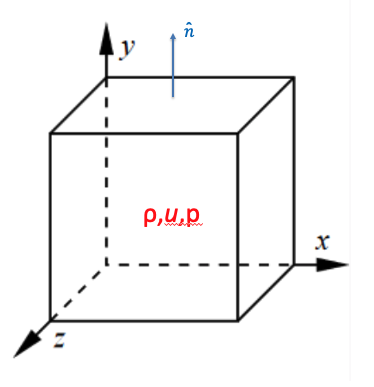
\includegraphics{./figs/controlvolume.jpg}}
  \end{center}
  \caption[]{For control volume we consider a cube of unit length, a
    3D generalization of the fluid patch. The
    volume is homogeneus and uniform: it has constant density $\rho$, velocity $\v{u}$, and pressure
    $p$. }
  \label{fig:controlvolume}
\end{figure}


\subsection{Mass Conservation}

The time rate of change of the mass contained in the volume $V$ is equal to the (negative)
value of the mass flux $\rho \v{u}$ across the surface (with $\rho$ and $\v{u}$ denoting the mass density and
flow velocity, respectively)

\beq
\frac{d}{dt} \int_V \rho dV = -\oint_A \rho \v{u}\cdot d\v{A} 
\eeq

This expression states that the control volume can only lose or gain
mass if this mass crosses the boundary of the volume. There is no mass
creation or anihilation. The lion cannot magically disappear from the
cage. It has to walk out of it. Using now the divergence theorem 

\beq
\frac{d}{dt} \int_V \rho dV = -\int_V \Div{\left(\rho\v{u}\right)}dV
\eeq

\noindent Given that $V$ is fixed, so we can write

\beq
\int_V \left[\ptderiv{\rho} + \Div{\left(\rho\v{u}\right)}\right]dV = 0 
\eeq

\noindent and since $V$ is completely arbitrary, the integrand must vanish. Thus we obtain the
equation of continuity:

\beq
\ptderiv{\rho} + \Div{\left(\rho\v{u}\right)} = 0
\label{eq:continuity-conservative}
\eeq


Often it is useful to write such equations in index notation 

\beq
\partial_t\rho + \partial_j \left(\rho u_j\right) = 0 
\eeq

\classcomm{if anyone asks, in putting the differentiation inside the integral,
we're using Leibniz Integral rule: \[
\frac{d}{dt} \left(\int_{a(t)}^{b(t)} f(x,t) dx\right) =
\int_{a(t)}^{b(t)} \frac{\partial}{\partial t}f(x,t) dx + f(b(t),t)
\frac{d}{dt}b(t) - f(a(t),t) \frac{d}{dt}a(t)
\]
\\
If the functions 
$a(t)$ and $b(t)$ are constant, $a(t)=a$ and $b(t)=b$
this simplifies to
\\
\[
\frac{d}{dt} \left(\int_{a}^{b} f(x,t) dx\right) =
\int_{a}^{b} \frac{\partial}{\partial t}f(x,t) dx 
\]
}

\subsection{Momentum Conservation}

The time rate of change of the fluid momentum in volume $V$ equals the surface integral
of the momentum flux due to fluid flow across $A$, plus the effect of the pressure $p$ acting
on the fluid across the surface $A$, plus the contribution of external forces (e.g. gravity)
acting on every point of $V$ (causing an acceleration $\v{f}$):

\beq
\frac{d}{dt} \int_V \left(\rho \v{u}\right) dV = -\oint_A \left(\rho  \v{u}\right)\v{u}\cdot d\v{A} - \oint_A \vt{P} \cdot d\v{A}  +\int_V \rho\v{f} dV
\eeq

Applying the divergence theorem to transform the surface integrals into volume integrals
we obtain 

\beq
\int_V \left[\ptderiv{\left(\rho \v{u}\right)} + \Div{ \left(\rho  \v{u}\otimes\v{u}\right)} +\Div{\vt{P}}  - \rho\v{f} \right]dV = 0 
\eeq

For a scalar pressure, $\vt{P}=p\vt{I}$, and we have
$\Div{\vt{P}}=\grad{p}$, writing 

\beq
\int_V \left[\ptderiv{\left(\rho \v{u}\right)} + \Div{ \left(\rho  \v{u}\otimes\v{u}\right)} +\grad{p}  - \rho\v{f} \right]dV = 0 
\eeq

\noindent again since the volume $V$ is completely arbitrary, the integrand must
vanish. We obtain the momentum equation. 

\beq
\ptderiv{\left(\rho \v{u}\right)} + \Div{ \left(\rho\v{u}\otimes\v{u}\right)} = -\grad{p} + \rho\v{f}
\label{eq:momentum-conservative}
\eeq

\classcomm{A few notes on this, since students may not be familiar with the
$\otimes$ operator, and index notation can be a problem. Explain it as
the external product $\v{a}\otimes\v{b} = \v{a}:\v{b} = a_ib_j$}

\begin{figure}
  \begin{center}
    \resizebox{.5\textwidth}{!}{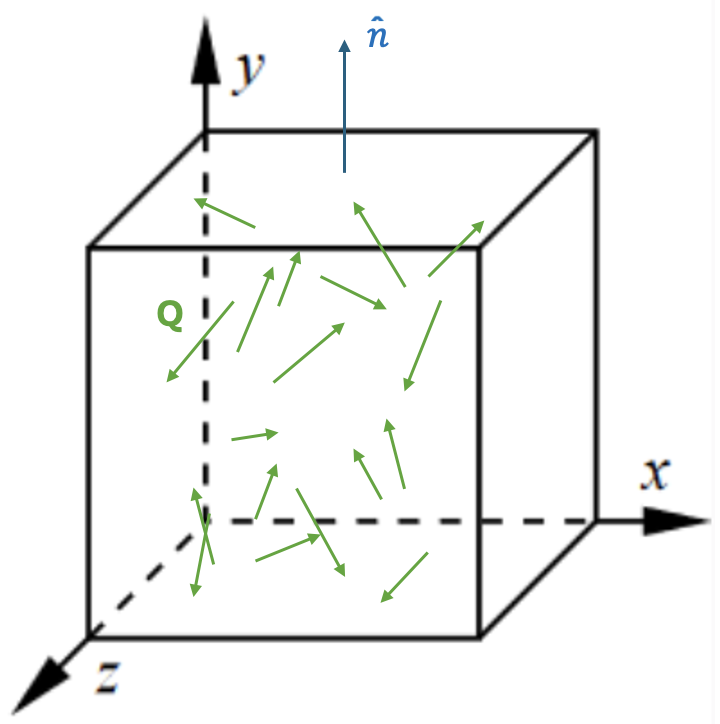
\includegraphics{./figs/momentumflux.png}}
  \end{center}
  \caption[]{A vector $\v{Q}$ flows in or out of the control volume
    with flux rate given by $\v{Q}\otimes\v{u}$. In index notation, $\v{Q}\otimes\v{u}$ is the
tensor $\vt{C}$ with components $C_{ij} = Q_i u_j$. It means the component $i$ of the
vector $\v{Q}$ flowing in the direction $j$}
  \label{fig:momentumflux}
\end{figure}

Notice that the term $\rho\v{u}\otimes\v{u}$ is the momentum flux.
Consider any vector field $\v{Q}$ (shown in green inside the cube in \fig{fig:momentumflux}).
The interpretation of $\v{Q}\otimes\v{u}$ as the flux of $\v{Q}$ is intuitive, though in this
case $\v{Q}\otimes\v{u}$ has to be a 2nd rank tensor. In index notation, $\v{Q}\otimes\v{u}$ is the
tensor $\vt{C}$ with components $C_{ij} = Q_i u_j$. It means the component $i$ of the
vector $\v{Q}$ flowing in the direction $j$.
The vector $\v{Q}$ flows in all directions. It is only the flux normal to the
area that flows in/out of the box.
Substituting $\v{Q}=\rho\v{u}$ does not change this interpretation. It adds,
however, the non-intuitive notion that {\it the velocity advects itself}. This
is a manifestation of Newton’s first law: an object in motion remains
in motion.

In index notation, the momentum equation is

\beq
\partial_t\left(\rho u_i\right) + \partial_j \left(\rho u_iu_j\right)=-\partial_i p + \rho f_i
\eeq

Notice how we can write the unit tensor $\vt{I}$ in index notation as
$\delta_{ij}$, the Kronecker delta. In this notation, the pressure
tensor is $P_{ij}$, which reduces to $p\delta_{ij}$ for scalar
pressure. Due to index summation rules

\beq
\partial_j P_{ij} = \partial_j p \delta_{ij} = \partial_i p
\eeq

\noindent which is what we wrote to replace the divergence of the tensor
pressure by the gradient of the scalar pressure. Keeping the tensor
pressure

\beq
\partial_t\left(\rho u_i\right) + \partial_j \left(\rho u_iu_j + P_{ij}\right)= \rho f_i
\eeq

\noindent we refer to the quantity $\rho u_iu_j + P_{ij}$ as the {\it Cauchy
  stress tensor}, or simply the stress tensor of the fluid. From the
conservation definition, the stress tensor is the momentum flux of the
fluid. 

Usually, $P_{ij}$ is due to random thermal motion. As we will see, with
an equation of state for ideal gases, $P_{ij}=p\delta{ij}=\rho c_s^2$, where
$c_s$ is the sound speed, which is of order of the mean thermal speed
of the molecules. The first term $\rho u_iu_j$ has dimension of
pressure, and is sometimes called the {\it ram pressure}. It's the
pressure caused by the bulk motion of the fluid. The galaxy NGC 4402
\figp{fig:rampressure-galaxy} is an example of this ram pressure in
astrophysical context. The galaxy is falling into the Virgo
cluster, and undergoing ram pressure stripping by the intracluster
medium (ICM), which is high pressure (hot and dense).

\begin{figure}
  \begin{center}
    \resizebox{\textwidth}{!}{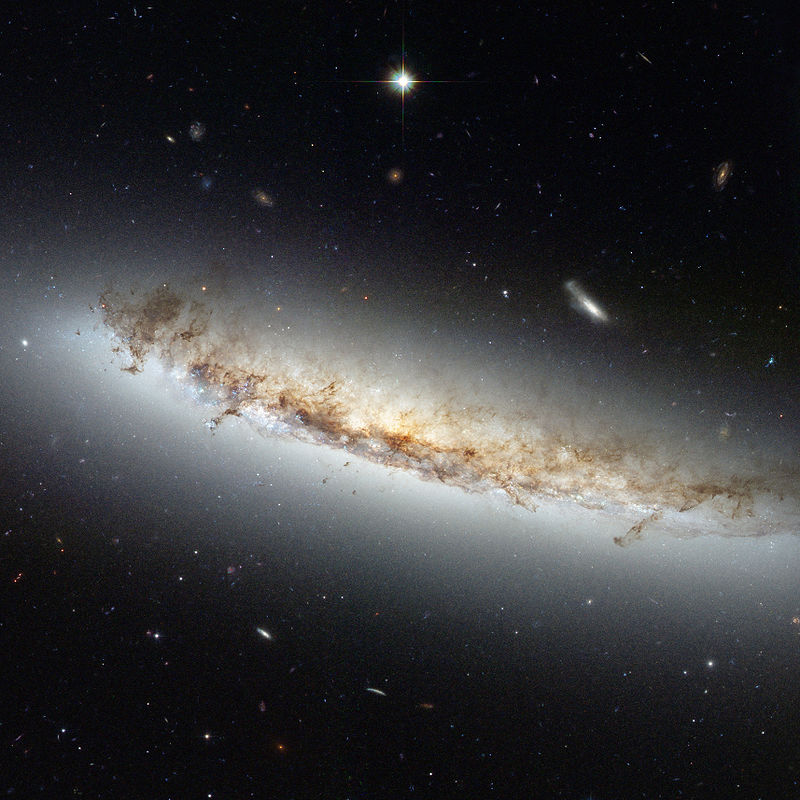
\includegraphics{./figs/NGC4402_ram_pressure.jpg}}
  \end{center}
  \caption[]{NGC 4402. The galaxy is falling into the Virgo
cluster, and undergoing ram pressure stripping by the intracluster
medium (ICM), which is high pressure (hot and dense). Credit: ESA/Hubble.}
  \label{fig:rampressure-galaxy}
\end{figure}


\section{Energy conservation}

The time rate of change of the total fluid energy (kinetic energy of fluid motion plus
internal energy, where $e$ denotes the specific internal energy) equals the surface integral
of the energy flux (kinetic + internal), plus the surface integral of the work done by the
pressure plus the volume integral of the work done by external forces

\beq
\frac{d}{dt} \int_V \left(\frac{\rho u^2}{2}+\rho e\right) dV =
-\oint_A \left(\frac{\rho u^2}{2}+\rho e\right)\v{u}\cdot d\v{A} -
\oint_A \v{u}\cdot \left(\vt{P} \cdot d\v{A}\right)  +\int_V \rho \v{u}\cdot\v{f} dV
\eeq

\classcomm{If the students get confused by the $\v{u}\cdot \left(\vt{P} \cdot
  d\v{A}\right)$ term, write in terms of $u_i
p\delta_{ij}\hat{n}_jdA$. Or explain qualitatively: the force is
$pdA$, so $u pdA$ is the work done by (or against) the force.}

Using the divergence theorem we obtain the total energy equation:

\beq
\frac{\partial}{\partial t} \left(\frac{\rho u^2}{2}+\rho e\right)  +
\Div{\left[\left(\frac{\rho u^2}{2}+\rho e\right)\v{u}\right]} = -\Div{\left(p\v{u}\right)}+\rho \v{u}\cdot\v{f}
\eeq

Calling the total energy

\beq
E = \frac{\rho u^2}{2}+\rho e
\eeq

\noindent we have the form originally introduced

\beq
\frac{\partial E}{\partial t} +
\Div{\left(E\v{u}\right)} = -\Div{\left(p\v{u}\right)}+\rho \v{u}\cdot\v{f}
\eeq

\noindent notice that we can add the pressure into the divergence on the left
hand side, 

\beq
\frac{\partial E}{\partial t} +
\Div{\left[\left(E+p\right)\v{u}\right]} =\rho \v{u}\cdot\v{f}
\label{eq:energy-conservative}
\eeq

\noindent which obviates that $\left(E+p\right)\v{u}$ is the energy flux in the fluid. 

\classcomm{Highlight that there are many forms of energy. Here we only
considered thermal and kinetic, but the ``full'' energy can contain
radiation force, magnetic force, etc. Many times it will be useful to
consider only the evolution of the thermal energy alone, since all
other forms of energy can be derived from the evolution equation of
their respective quantities (kinetic from $\v{u}$, magnetic from
$\v{B}$, etc). Evolving the total energy is important for conservative
methods, but non-conservative methods can simply evolve the internal
energy (or any other thermodynamic variable).}

\subsection{External forces}

Typically in astrophysics, a common external force is gravity. In this
case $\v{f}=\v{g}$, and $\v{g}$ is given by Poisson's equation

\beq
\Div{\v{g}}=-4\pi G \rho 
\eeq

Another common force is radiation pressure. In this case, the
acceleration is 

\beq
\v{f}_{\rm rad} = \frac{1}{c} \int \kappa_\nu \v{F}_\nu d\nu 
\eeq

With these, the equations become

\begin{eqnarray}
  \ptderiv{\rho} + \Div{\left(\rho \v{u}\right)} &=& 0 \\
\ptderiv{\left(\rho \v{u}\right)} + \Div{\left(\rho
  \v{u}\otimes\v{u}\right)} &=& -\grad{p} + \rho\v{g} + \rho\v{f}_{\rm rad}\\
\ptderiv{E} + \Div{\left(E\v{u}\right)} &=& -\Div{\left(p\v{u}\right)}
                                            + \rho\v{u}\cdot\v{g}+
                                            \rho\v{u}\cdot\v{f}_{\rm
                                            rad} + \mathcal{H} -\mathcal{C} 
  \end{eqnarray}

\noindent where we also added heating and cooling by radiation.

\section{Eulerian and Lagragian forms of the equations of motion}

\begin{figure}
  \begin{center}
    \resizebox{\textwidth}{!}{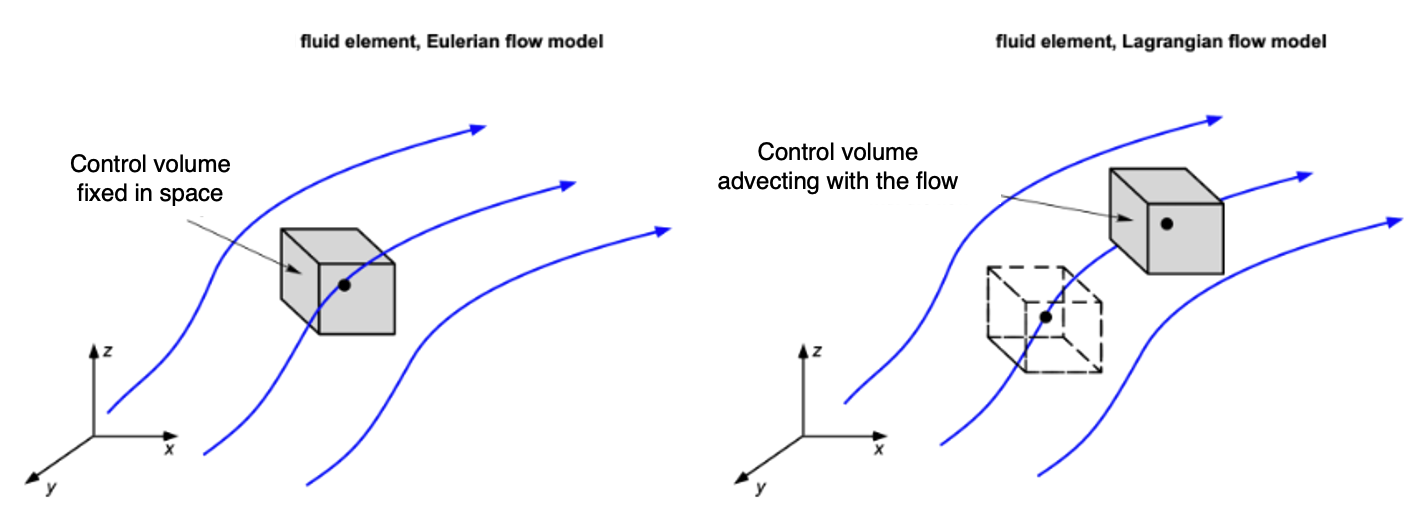
\includegraphics{./figs/EulerianLagrangian.png}}
  \end{center}
  \caption[]{Eulerian vs Lagrangian formulation. Reproduced from
    \cite{Leishman}.}
  \label{fig:eulerian-lagrangian}
\end{figure}

The equations derived in this form so far are useful as they are in
conservative form, evidencing what quantity is being conserved and
how. This is also useful for numerical hydrodynamics that use
conservative schemes. However, there are other ways to think of
hydrodynamic, which can give other useful intuitive insights. The
{\it Eulerian} derivative $\partial_t$ means derivation in time at a
fixed point. The flow is sampled with points and one looks at how the
quantities vary at that point (left panel of \fig{fig:eulerian-lagrangian}). We can also think of following a fluid
parcel itself, which is flowing with velocity $\v{u}$, and follow the
time evolution in the co-moving frame of this parcel. This is the {\it
  Lagrangian} derivative (right panel of \fig{fig:eulerian-lagrangian}). They are related by 

\beq
\frac{D}{D t} = \ptderiv{} + \v{u}\cdot \grad
\eeq

This is called co-moving derivative, advective derivative, full
derivative, Lagrangian derivative, material derivative, total
derivative, ``convective'' derivative, etc.

We will solve later in the semester the 1D advection equation numerically

\beq
\ptderiv{f(x,t)} = - u \frac{\partial f(x,t)}{\partial x}
\eeq

The solution of this equation is $f(x,t) = f(x-ut,0)$. This represents
a wave or profile that moves without distortion at a constant velocity
$u$. 

Proof: If $u$ is constant, then a Galilean transformation $x\rightarrow x-ut$ should
leave the system unchanged. That means that a function $f$ is constant
along lines of $x-ut\equiv{\rm const}$. We can then define a function
$g$ such that 

\beq
f(x,t) = g(x-ut)
\label{eq:fxt}
\eeq

Notice that by doing this transformation, the PDE became an ODE. We
say that $x-ut$ is a  {\it characteristic curve}.

Setting $t=0$, we have $f(x,0) = g(x)$, which means that $g(x)$ is the
initial condition of $f$. Since x is a dummy variable, $f(x-ut,0) =
g(x-ut)$. Substituting \eq{eq:fxt} completes the proof, $f(x,t)=f(x-ut,0)$.


\subsection{Continuity equation in Lagrangian form}

The continuity equation is simple to put in Langrangian form, simply
expand the divergence 

\beq
  \ptderiv{\rho} + \left(\v{u}\cdot \grad\right)\rho= - \rho \Div{\v{u}}
\eeq

\noindent or 

\beq
  \frac{D\rho}{Dt} = - \rho \Div{\v{u}}
\eeq

This form of the continuity equation has a physical meaning. It says that a gas parcel changes
its density when the gas motion converges. In other words: when the gas motion is such that the
parcel gets compressed. This compression is expressed as the negative
of the divergence $-\Div{\v{u}}$. This is shown in \fig{fig:compression}.

\begin{figure}
  \begin{center}
    \resizebox{\textwidth}{!}{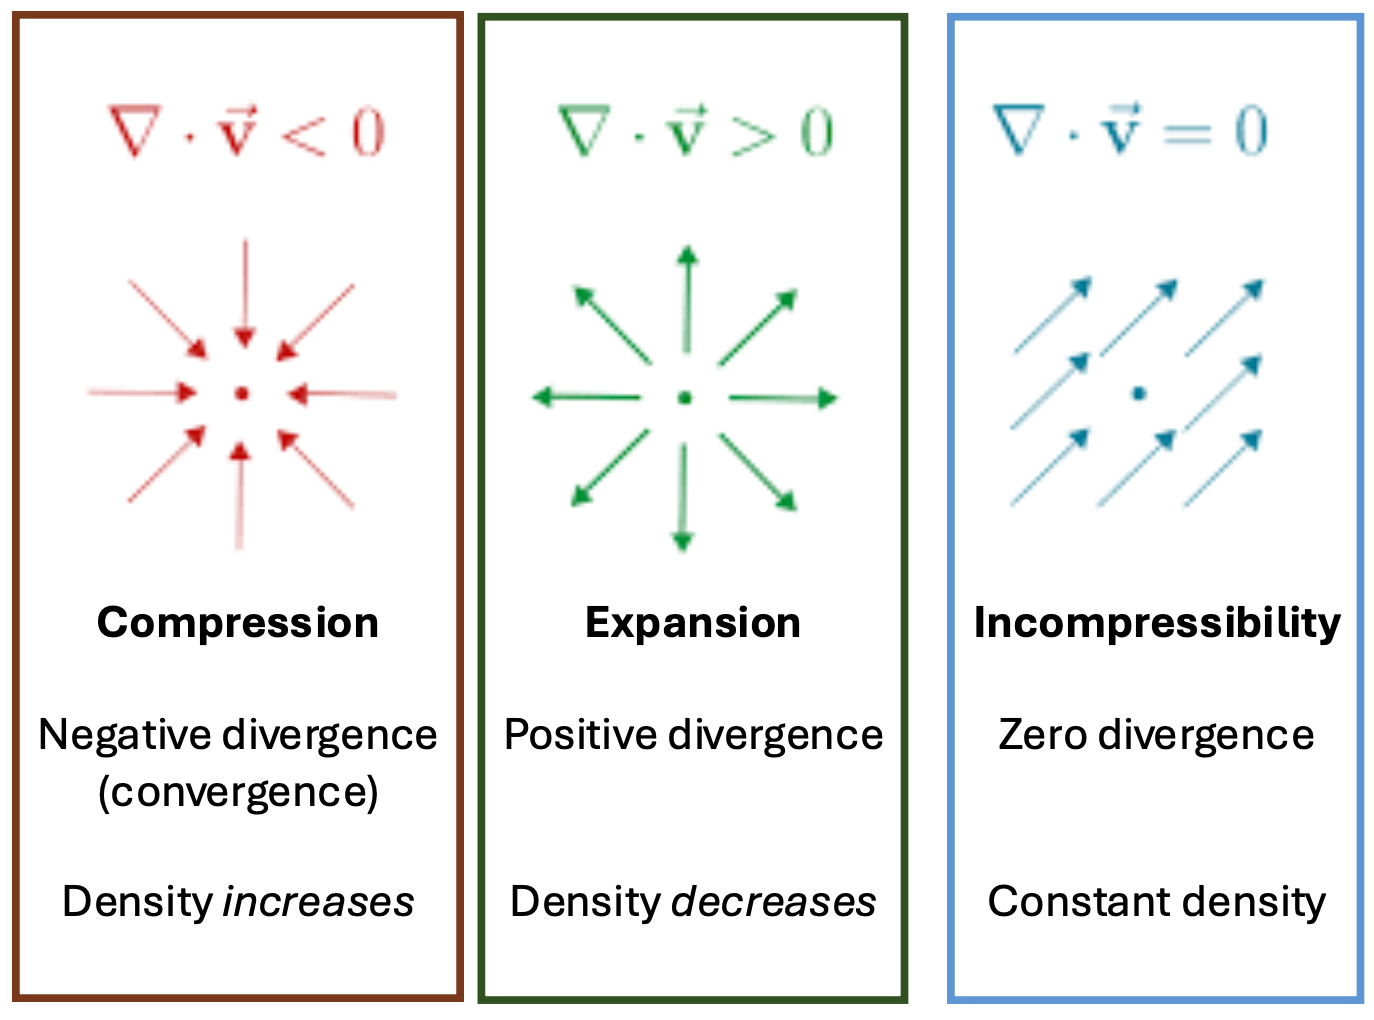
\includegraphics{./figs/compression.png}}
  \end{center}
  \caption[]{The effect of the compression term in the continuity equation.}
  \label{fig:compression}
\end{figure}



\subsection{Momentum equation in Lagrangian form: Euler equation}

Consider the momentum equation, dropping the external acceleration 


\beq
\ptderiv{\left(\rho \v{u}\right)} + \Div{ \left(\rho\v{u}\otimes\v{u}\right)} = -\grad{p} 
\eeq

\noindent and expand the first term 

\beq
\rho\ptderiv{\v{u}} +\v{u}\ptderiv{\rho} + \Div{ \left(\rho\v{u}\otimes\v{u}\right)} = -\grad{p} 
\eeq

\noindent and also expand the divergence

\beq
\Div{\left(\rho  \v{u}\otimes\v{u}\right)} = \v{u}\Div{\left(\rho\v{u}\right)} +\rho \left(\v{u}\cdot  \grad\right) \v{u}
\eeq

\classcomm{if they don't know this, do the dot product in index
notation: $\partial_j \left(\rho u_i u_j\right) = u_i\partial_j \left(\rho  u_j\right) + \rho u_j \partial_j u_i$
}

So we find 

\beq
\rho\ptderiv{\v{u}} +\v{u}\ptderiv{\rho} +
\v{u}\Div{\left(\rho\v{u}\right)} +\rho \left(\v{u}\cdot  \grad\right)
\v{u} = -\grad{p} 
\eeq

\noindent the two middle terms cancel because of the continuity equation

\beq
\rho\ptderiv{\v{u}} +\v{u}\cancel{\left[\ptderiv{\rho} +\Div{\left(\rho\v{u}\right)}\right]} +\rho \left(\v{u}\cdot  \grad\right)
\v{u} = -\grad{p} 
\eeq

\noindent dividing by $\rho$, this leaves

\beq
\ptderiv{\v{u}} +\left(\v{u}\cdot  \grad\right) \v{u} = -\frac{1}{\rho}\grad{p} 
\eeq

\noindent or, using the advective derivative

\beq
\frac{D\v{u}}{Dt} = -\frac{1}{\rho}\grad{p} 
\label{eq:euler-lagrangian}
\eeq

This form of the equation of momentum conservation also has a physical interpretation. It says
that a gas parcel will be accelerated due to a force, which is the pressure gradient. Any other
body force, such as gravity, can be easily added as a term on the
right-hand-side. In other words, Euler's equation is simply
$\v{F}=m\v{a}$ for fluids. Write 

\beq
\v{a} = \frac{D\v{u}}{dt} = \frac{\partial \v{u}}{\partial t} + \left(\v{u}\cdot\del\right)\v{u}
\label{eq:aadvec}
\eeq

\noindent for a volume element and considering only pressure, the
force acting on it, we have seen is $d\v{F}=-\vt{P}\cdot dA$, which
we can use Gauss theorem and $\vt{P}=p\delta_{ij}$ to find
$d\v{F}-\grad{p}dV$. Equating that to  $d\v{F}=dm \v{a}$, we find 

\beq
\v{a} = -\grad{p}\frac{dV}{dm}
\eeq

\noindent substituting $dm=\rho dV$ and \eq{eq:aadvec}, we find
\eq{eq:euler-lagrangian}. The conclusion is an
equivalence between Euler's equation and Newton's 2nd law.

\subsection{Energy equation in Lagrangian form}

Given the energy equation 

\beq
\ptderiv{E} + \Div{\left(E\v{u}\right)} = -\Div{\left(p\v{u}\right)} +
\rho\v{u}\cdot \v{f}
\eeq

\noindent we expand the divergence in the left hand side first 

\beq
\ptderiv{E} +(\v{u}\cdot\grad)E + E\Div{\v{u}}  =-\Div{\left(p\v{u}\right)} + \rho\v{u}\cdot \v{f}
\eeq

\noindent group the first terms in a Lagrangian derivative

\beq
\frac{DE}{Dt} + E\Div{\v{u}}  = -\Div{\left(p\v{u}\right)}+\rho\v{u}\cdot \v{f}
\eeq

\noindent and now expand $E=\rho e + \rho u^2/2  = \rho e_{\rm tot}$, where $ e_{\rm
  tot}=e + u^2/2$ is the sum of (specific) internal and kinetic
energies. 

\beq
\rho\frac{De_{\rm tot}}{Dt} + e_{\rm tot}\frac{D\rho}{Dt} + e_{\rm tot}\rho\Div{\v{u}}  = -\Div{\left(p\v{u}\right)} +\rho\v{u}\cdot \v{f}
\eeq

\noindent again the middle terms cancel because of the continuity equation, so 

\beq
\frac{De_{\rm tot}}{Dt}  = -\frac{1}{\rho}\Div{\left(p\v{u}\right)}+\v{u}\cdot \v{f}
\eeq

Given $ e_{\rm  tot}=e + u^2/2 = e + \v{u}\cdot\v{u}/2$ (or use $u_ju_j$), we can write 

\beq
\frac{De}{Dt} + \v{u} \cdot\frac{D\v{u}}{Dt} = -\frac{1}{\rho}\Div{\left(p\v{u}\right)}+\rho\v{u}\cdot \v{f}
\eeq

\noindent expanding the divergence in the right hand side 

\beq
\frac{De}{Dt} + \v{u} \cdot\frac{D\v{u}}{Dt} =-\frac{p}{\rho}\Div{\v{u}} -\frac{1}{\rho}\v{u} \cdot \grad p+\rho\v{u}\cdot \v{f}
\eeq

Grouping the terms dotted with $\v{u}$ 

\beq
\frac{De}{Dt} + \v{u} \cdot \left[\frac{D\v{u}}{Dt} +\frac{1}{\rho}\v{u} \cdot \grad p-\rho\v{u}\cdot \v{f} \right]=-\frac{p}{\rho}\Div{\v{u}} 
\eeq

\noindent the term in brackets is simply the momentum equation, so they
cancel. That is, we're canceling out all kinetic terms and leaving
only the internal energy. This leaves


\beq
\frac{De}{Dt} = -\frac{p}{\rho}\Div{\v{u}} 
\eeq

This also has physical meaning: the thermal energy of a gas parcel changes only as a result of
adiabatic compression. This is the pdV work. Notice how the work of body forces
will not change the internal energy, only the kinetic. 

\subsubsection{Entropy equation}

Recall that the first law of thermodynamics. If we have a fluid in thermodynamic
equilibrium to which some amount of heat $dQ$ has been added, then

\beq
dQ = d U + d W
\label{eq:first-law-thermo}
\eeq

\noindent where $dU$ is the change in energy and $dW=p dV$ is the work done
by the system. This does not apply for the fluid as a whole (the
entire system is not in thermodynamic equilibrium), but can be applied
to a fluid patch. Yet, these quantities all have unit of erg, that is, they're the
energy, not the specific energy $e$ (energy per gram). 

Let this fluid element have mass $ m$, and define $dQ =  m
dq$ and $dU = m de$. Since $V = m / \rho$, then
$dV=-m/\rho^2 d\rho$. Putting together, and dividing by mass 

\beq
dq = de - \frac{p}{\rho^2} \rho
\label{eq:first-law-thermo}
\eeq

\noindent Now substituting $dq=Tds$ 

\beq
Tds  = de - \frac{p}{\rho^2} \rho 
\eeq

\noindent where $s$ is the entropy. Dividing by $dt$

\beq
T\frac{Ds}{Dt}  = \frac{De}{Dt} - \frac{p}{\rho^2} \frac{D\rho}{Dt}
\eeq

\noindent substituting by the continuity equation 

\beq
T\frac{Ds}{Dt}  = \frac{De}{Dt} + \frac{p}{\rho} \Div{\v{u}}
\eeq

\noindent Comparing with the equation obtained, implies 

\beq
\frac{Ds}{Dt}=0
\eeq

\noindent or to say: the entropy of a gas parcel does not change along
its path of motion! The equations of hydrodynamics, at least the
simplified forms we wrote down until now, conserve entropy.
After its journey, a fluid parcel lies on the same adiabat as it started out.

This statement is only true if there is no heating or cooling. Heating or cooling
affect the entropy. So will shocks, which do not conserve entropy.

A simple heat exchange is to consider that the heat flux $\v{F}$ inside a
fluid can usually be assumed to follow Fick's law, i.e., proportional
to the gradient, 

\beq
\v{F} = -K\grad{T}
\eeq

\noindent where $K$ is the coefficient of thermal conductivity (units erg s$^{-1}$cm$^{-1}$ K$^{-1}$). The heat loss
rate from a volume is the heat flux integrated over the surface

\beq
\oint \v{F}\cdot d\v{A} = \int  \Div{\v{F}} dV
\eeq

\noindent Notice that $\Div{\v{F}}$ has units of erg s$^{-1}$
cm$^{-3}$. Thus the heat gain and loss that
we called $H-C$ (in units of erg s$^{-1}$ g$^{-1}$) in the energy equation is 
$\rho^{-1}\Div{\v{F}}$

\beq
\frac{De}{Dt} = - \frac{p}{\rho} \Div{\v{u}} -\frac{1}{\rho}\Div{\v{F}}
\eeq

For the case considered, this term simply becomes $K\Laplace{T}$. For
incompressible fluids, this becomes 

\beq
\rho\frac{De}{Dt} = K\Laplace{T}
\eeq

For no bulk flows in 1D (so Eulerian=Lagrangian, canceling the
$\v{u}\cdot\del$ term), and considering $e=c_v T$, this becomes the
celebrated heat equation

\beq
\frac{\partial T(x,t)}{\partial t} = \chi \frac{\partial^2 T(x,t)}{\partial x^2}
\eeq

\noindent where $\chi = K/c_v \rho$ is the coefficient of thermal
diffusivity.  

The steady-state equilibrium solution is to
zero to the second derivative, i.e., constant gradient. Valleys are
filled, peaks are eroded. So is the nature of diffusion: it tends to
smooth gradients. 

In astrophysics diffusion processes tend to be slow, because the
dimensions are too large, but diffusion is important numerically, and
many planetary processes are diffusion-dominated. Heat transport in
astrophysics is often radiative, in which case the energy flux $\v{F}$ is
the usual flux from radiative transfer theory. 

\subsection{Solution of Diffusion Equation}

Considering

\beq
\frac{\partial f(x,t)}{\partial t} = D \frac{\partial^2 f(x,t)}{\partial x^2}
\eeq

With initial condition $f(x,0)=\delta(x)$ and boundary conditions
$f(-\infty,t)=f(\infty,t)=0$. We solve this by Fourier transforms

\beqn
f(k,t) &=& \int f(x,t) e^{ikx} dx \label{eq:fourier-kx}\\
f(x,t) &=& \frac{1}{2\pi}\int f(k,t) e^{-ikx} dk \label{eq:fourier-xk}
\eeqn

%applying $f(x,0)$, we find $f(k,0)=1$.

We plug \eq{eq:fourier-xk} this into the diffusion equation to find
the diffusion equation in Fourier space

\beq
\int \left[\frac{\partial f(k,t)}{\partial t} +Dk^2 f(k,t) \right]e^{-ikx} dk =0
\eeq

\noindent the integrand has to be zero, so we can solve it for
$f(k,t)$, finding 

\beq
f(k,t)=e^{-Dk^2t}
\eeq

Now we apply \eq{eq:fourier-xk} again to find $f(x,t)$

\beq
f(x,t) = \frac{1}{2\pi}\int e^{-Dk^2t} e^{-ikx} dk 
\eeq

The sympy code to find this integral is

\begin{mintedbox}{python}
import sympy as sp

x,k = sp.symbols('x k',real=True)
t,D = sp.symbols('t D',real=True,positive=True)

integrand = sp.exp(-(D*k**2*t + sp.I*k*x))/2/sp.pi

f = sp.integrate(integrand,(k,-sp.oo,sp.oo))

print("f(x,t)=",sp.simplify(f))
\end{mintedbox} 

\noindent which yields

\beq
f(x,t) = \frac{1}{2\sqrt{\pi Dt}}e^{-\frac{x^2}{4Dt}}
\eeq

The $t=0$ value indeed is a Dirac's delta, justifying the
initial condition. The normal distribution is 

\beq
g(x) = \frac{1}{\sqrt{2\pi}\sigma} e^{-\frac{x^2}{2\sigma^2}}
\eeq

So the solution is a Gaussian with $\sigma(t)=\sqrt{2Dt}$, i.e., the amplitude
decreasing in time, and width increasing in time.  

\begin{figure}
  \begin{center}
    \resizebox{\textwidth}{!}{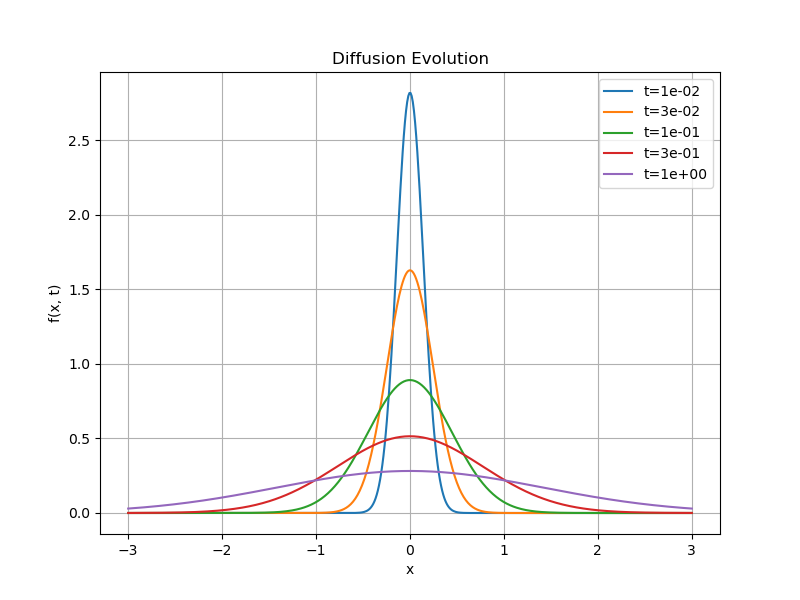
\includegraphics{./figs/Gaussian_Spreading.png}}
  \end{center}
  \caption[]{Diffusion solutions at different times.}
  \label{fig:diffusion}
\end{figure}

\classcomm{Do a chapter or subchapter with the thermodynamics.}

\section{Viscosity}

Viscosity and heat diffusion are two sides of the same
coin. Microphysically, molecules exchange heat as they pass from one
fluid element to another within a mean-free path. Similarly, they also
exchange momentum. This diffusion of momentum is called viscosity. 

The fact that the mean free path is small but finite has the consequence
that particles can be exchanged between adjacent fluid elements, which
creates transfers of momentum and energy in addition to those that we
have studied in the previous sections. This is the origin of dissipative
processes such as viscosity and thermal conduction.

Viscosity creates forces that tend to prevent velocity gradients, i.e.
it is a force that opposes layers moving relative to each other. We
can add this force in the stress tensor as described below. 

\begin{figure}
  \begin{center}
    \resizebox{.5\textwidth}{!}{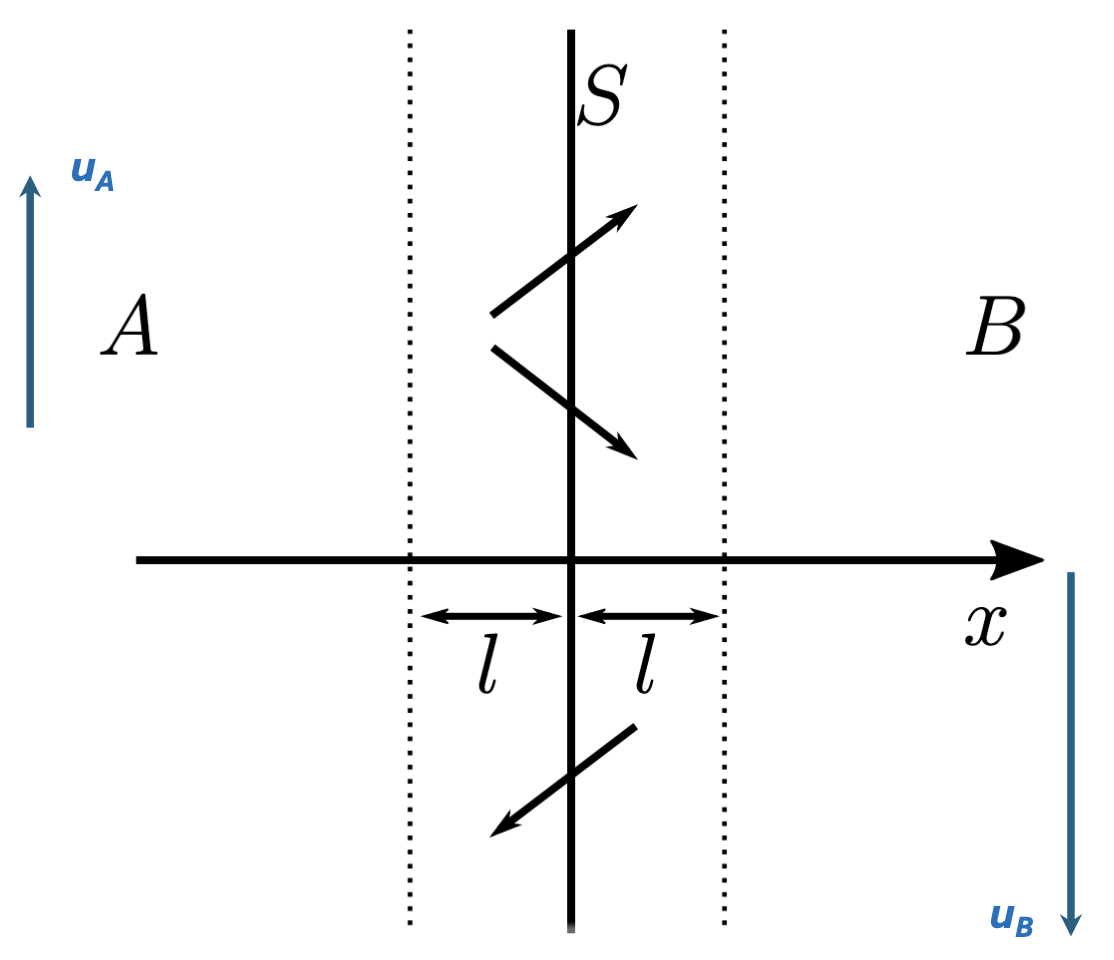
\includegraphics{./figs/viscosity.png}}
  \end{center}
  \caption[]{Particles exchanged between adjacent fluid elements A and
    B are the origin of viscosity. Molecules are exchanged between layers whose thickness is of the order of the
    mean free path $l$. Fluid elements are much bigger than $l$. If Aand B are moving in
    the $y$ direction with different velocities, particles escaping from the faster fluid
    element will accelerate the slower one and viceversa. Reproduced
    from \cite{Sormani22}.}
  \label{fig:viscosity}
\end{figure}

We saw that the surface force acting on a fluid must be related
through a second rank tensor, $P_{ij}$

\beq
\left(d\v{F}_{\rm surface}\right)_i = P_{ij} dA_j
\eeq

\noindent and the total surface force is found by integrating over all the area
elements

\beq
\v{F}_{{\rm surface},i} = \oint P_{ij} dA_j
\eeq

\noindent which when integrated yields a divergence of the tensor. For a scalar,
that becomes a gradient, the pressure gradient force. However, that's
just the diagonal of the tensor. If the full surface was only
diagonal, then only vertical forces to a surface would occur. Yet, if
a fluid has internal friction (which in fluids we call viscosity), a
tangential force to the surface must also happen \classcomm{Show slide
  with pressure and stress}. 

In general, a full second-rank
tensor should satisfy this requirement, so that

\beq
P_{ij}=p\delta_{ij} + \pi_{ij}
\eeq

For an ideal fluid, $\pi_{ij}=0$, so there's no
viscosity. \classcomm{Show slide with shear flow}. If there is
internal friction, a force will be communicated from the faster part
of the flow to the slower part of the flow, accelerating it to try to
neutralize the shear. \classcomm{Give the definition of shear:} Shear is a velocity gradient in a different
direction:

\beq
\frac{\partial u_i}{\partial x_j}
\eeq

This force has to act accross the surface, yet tangentially to the surface. Mathematically,
this can only be realized if $\pi_{ij}$ has off-diagonal elements. The
shear force is expected to be larger the larger the shear is. Based on
this intuition, Newton
postulated that the shear force should be proportional to the
velocity gradient. The most general second-rank tensor that can be
constructed out of velocity gradients is 

%\beq
%\pi_{xy} = -\mu \frac{\partial u_x}{\partial y}
%\eeq

\beq
\pi_{ij} = a \left(\frac{\partial u_i}{\partial x_j}+\frac{\partial u_j}{\partial x_i}\right)+b\delta_{ij}\Div{\v{u}}
\eeq

\noindent and given that all the isotropic part of the stress tensor is given by
$p\delta_{ij}$, $\pi_{ij}$ needs to be traceless (otherwise it would give
normal forces). $\pi_{ij}$ will be traceless if $b=-2a/3$, so we find 

\beq
\pi_{ij} = -\mu \left(\frac{\partial u_i}{\partial x_j}+\frac{\partial u_j}{\partial x_i}-\frac{2}{3}\delta_{ij}\Div{\v{u}}\right)
\eeq

\noindent with $\mu$ being the viscosity coefficient. A fluid that obey this proportionality between the shear stress and the
velocity gradient are called {\it Newtonian fluids}. In practice, most
flows are Newtonian. \classcomm{but show examples of non-Newtonian
  fluids and highlight that the origin of Non-Newtonian behavior is
  impurities in the fluid (cells for blood, macromolecules for starch,
  grains for colloids, etc.)} 

We can simplify the equations by defining the shear rate tensor
$\vt{S}$, given by 

\beq
S_{ij} = \frac{1}{2}\left(\frac{\partial u_i}{\partial x_j}+\frac{\partial u_j}{\partial x_i}-\frac{2}{3}\delta_{ij}\Div{\v{u}}\right)
\eeq


\noindent so that 

\beq
\vt{\pi} = -2\mu\vt{S}
\eeq

\noindent this tensor is also called rate-of-strain tensor. 


\subsection{Navier-Stokes equation}

Adding the viscous tensor to the momentum equation

\begin{equation}
\rho\frac{D u_i}{D t}  = -\frac{\partial p}{\partial x_i} +\rho f_i +
\frac{\partial }{\partial x_i}\left[ \mu\left(\frac{\partial
      u_i}{\partial x_j}+\frac{\partial u_j}{\partial
      x_i}-\frac{2}{3}\delta_{ij}\Div{\v{u}}\right)\right] 
\end{equation}


%\begin{equation}
%\rho\frac{D u_i}{D t}  = -\frac{\partial p}{\partial x_i} +\rho f_i +
%\frac{\partial }{\partial x_i}\left( 2\mu S_{ij}\right) 
%\end{equation}

%\begin{equation}
%\rho\frac{D \v{u}}{D t}  = -\grad{p} +\rho \v{f} -\Div{\left(2\mu\vt{S} \right)}
% \end{equation}

%\noindent defining $\mu= \rho\nu$, where $\nu$ is the kinematic viscosity ($\mu$
%is known as dynamical viscosity), and splitting the viscous term 

%\begin{equation}
%\frac{D \v{u}}{D t}  = -\frac{1}{\rho}\grad{p} +\v{f} +2\nu\Div{\left(\vt{S} \right)} +2\vt{S}\rho^{-1}\cdot\grad{\left(\nu\rho \right)}
% \end{equation}

\noindent splitting the terms

\begin{equation}
\rho\frac{D u_i}{D t}  = -\frac{\partial p}{\partial x_i} +\rho f_i +
\mu\frac{\partial }{\partial x_i}\left[ \left(\frac{\partial
      u_i}{\partial x_j}+\frac{\partial u_j}{\partial
      x_i}-\frac{2}{3}\delta_{ij}\Div{\v{u}}\right)\right]  + \frac{\partial \mu}{\partial x_i} \left(\frac{\partial
      u_i}{\partial x_j}+\frac{\partial u_j}{\partial
      x_i}-\frac{2}{3}\delta_{ij}\Div{\v{u}}\right)
\end{equation}

The 3rd term, with constant $\mu$, is evaluated in index notation

\beqn
\partial_j\partial_j u_i + \partial_i\partial_j u_j -\frac{2}{3}\partial_j\delta_{ij}\partial_k u_k &=& \partial_j\partial_j u_i + \partial_i\partial_j u_j -\frac{2}{3}\partial_i\partial_k u_k\\
&=&\Laplace \v{u} +\frac{1}{3}\grad{\left(\Div{\v{u}}\right)}
\eeqn

\noindent ignoring for the moment the case of varying viscosity, we can write 

\begin{equation}
\rho\frac{D \v{u}}{D t}  = -\grad{p} +\rho \v{f}+
\mu \left[\Laplace \v{u} +\frac{1}{3}\grad{\left(\Div{\v{u}}\right)}\right]
\end{equation}

\noindent and defining $\mu=\rho\nu$, where $\nu$ is the kinematic viscosity
($\mu$ is known as dynamical viscosity), 

\begin{equation}
\frac{D \v{u}}{D t}  = -\frac{1}{\rho}\grad{p} +\v{f} + 
\nu \left[\Laplace \v{u} +\frac{1}{3}\grad{\left(\Div{\v{u}}\right)}\right]
\end{equation}

The $\grad{\left(\Div{\v{u}}\right)}$ term is important for
variable compression (it is important, for instance, in dissipation of
acoustic waves). Yet, in many situations it can be ignored. In
this case, the Navier-Stokes equation takes a simplified form 

\begin{equation}
\frac{\partial \v{u}}{\partial t} +\left(\v{u}\cdot\del\right)\v{u}  = -\frac{1}{\rho}\grad{p} +\v{f} + 
\nu \Laplace \v{u} 
\end{equation}

The viscosity, at least in this approximation, behaves like diffusion
of momentum.  Though notice that the full equation


\begin{equation}
\frac{D \v{u}}{D t}  = -\frac{1}{\rho}\grad{p} +\v{f} +2\rho^{-1}\Div{\left(\mu\vt{S} \right)}
 \end{equation}

\noindent  leads to (show as homework)

\begin{equation}
\frac{D \v{u}}{D t}  = -\frac{1}{\rho}\grad{p} +\v{f} + \nu
\left[\Laplace \v{u} +\frac{1}{3}\grad{\left(\Div{\v{u}}\right)} + 2\vt{S}\cdot\grad\left(\ln\rho+\ln\nu\right)\right]
 \end{equation}

\noindent and the viscosity gradient can lead to non-diffusive effects. 
 
A few things to consider.

\begin{itemize}
  
\item nonlinear term: The NS equation has a nonlinear term in
  velocity, $\left(\v{u}\cdot\del\right)\v{u}$. The momentum advects
  itself. All the complex behavior of hydrodynamical flows comes from this term. Ultimately,
  this comes from Newton's 1st law, the law of inertia: an object
  remains in motion unless a force is applied to it. For an Eulerian
  description, it means that the flow will advect itself.

\item there is no general solution of the Navier-Stokes
  equation. You'll literally become a millionaire if you solve it. It
  is one of the seven
  \href{Millennium Prize
    problems}{https://www.claymath.org/millennium/navier-stokes-equation/}
  in mathematics. 

 \end{itemize}

 \subsection{Viscous heating}

 Having derived the viscous force, $-\Div{\vt{\pi}}$ we need to add the work done by the
 viscous force,  $-\v{u}\cdot\left(\Div{\vt{\pi}}\right)$ in the energy equation.

 \beq
\frac{DE}{Dt} = -u_i \partial_j\pi_{ij}
 \eeq

 Notice that

 \beq
\partial_ju_i \pi_{ij} = u_i\partial_j \pi_{ij} + \pi_{ij}\partial_j u_i 
 \eeq 

\noindent  so that

  \beqn
\frac{DE}{Dt} &=& -\partial_ju_i \pi_{ij} + \pi_{ij}\partial_j u_i \\
&=& \Div{\left(\v{u}\cdot\vt{\pi}\right)}-\left(\vt{\pi}\cdot\del\right)\v{u}
\eeqn

The first term is the viscous energy flux, as momentum in one
direction is diverted into another by the shear. The second is the kinetic
energy that is converted into heat. The viscous energy flux matters for kinetic
energy, but not for internal energy. The last term is a bona fide
heating term. We can see how this term is positive definite according
to the following analysis. Because $\partial_j u_i$ is symmetric, 

\beq
\partial_j u_i = \frac{1}{2}\left(\partial_j u_i+\partial_i u_j\right)
= S_{ij}+\frac{2}{3}\delta_{ij}\Div{\v{u}}
\eeq

\noindent substituting into the viscous heating

\beqn
-\pi_{ij}\partial_j u_i&=&2\mu S_{ij}\left(S_{ij}+\frac{2}{3}\delta_{ij}\Div{\v{u}}\right)\\
&=&2\mu \left(S_{ij} S_{ij}+\frac{2}{3}S_{ij}\delta_{ij}\Div{\v{u}}\right)
\eeqn

The second term is zero because $S_{ij}$ is traceless, so its inner
product with the Kronecker delta is zero. Thus, what is left is

\beq
-\pi_{ij}\partial_j u_i=2\mu \vt{S}^2
\eeq

\noindent which is positive definite. 

\section{Reynolds number}

When is viscosity important? To find out, we need to compare viscous
forces to other forces that are present in the fluid. Consider the
NS equation. The last term on the RHS are viscous forces,
while the LHS represents the total force acting on the fluid. Without fur-
ther information about the particular situation at hand, there is no way
to know which one is bigger. However, for a given situation we can often
estimate the relative contribution of these two terms and decide whether
we can neglect one of them. Suppose that in a particular situation fluid
quantities vary on a typical length scale $L$ and the flow has a typical
velocity $U$; for example, if we have an object moving in the fluid with
certain size and velocity this would give us some characteristics values.
Then we can crudely approximate the spatial derivatives as $\del \sim L^{-1}$.

The order of magnitude of the second term on the RHS of (125), which
represent viscous forces, is then

\beq
\frac{\nu U}{ L^2}
\eeq

\noindent while the order of magnitude of the term on the LHS is

\beq
\frac{U^2}{L}
\eeq


The ratio between the latter and the former is a dimensionless quantity
called the Reynolds number

\beq
\boxed{
  {\rm Re} = \frac{UL}{\nu}
  }
\eeq

The Reynolds number quantifies the relative impor-
tance of viscous forces and total (also called inertial, because they are
related with the total acceleration) forces.
A high Reynolds number corresponds to a flow in which viscous forces
are negligible. Such a flow may be smooth and steady, but, perhaps
counter-intuitively, is more often turbulent. A low Reynolds number, on the other hand,
corresponds to a viscosity-dominated flow, in which dissipational effects
damp out turbulence before it can become established.

In the vast majority of astrophysical flows, the Reynolds number is
very high, and viscosity can be neglected. For example, in the
interstellar medium the typical range is ${\rm Re} \sim 10^5$ to $10^{10}$.


What about the opposite regime, i.e. very low Reynolds numbers?
This gives us the chance for a little excursion. You may have never thought
about it, but there is a whole world where this regime is relevant. Since
microorganisms such as bacteria are small, their Reynolds numbers are
extremely small. For a bacteria, swimming through water is like for a human swimming in a pool of molasses while only being allowed to move at
1 cm/min, like the hands of a clock. The equations approximated for this
regime are completely different from the equations that are appropriate
in most astrophysical applications. In water, we can assume incompressibility and at bacteria scales we can through away the LHS in NS 
to obtain

\beq
0=-\grad{p} + \eta\Laplace{\v{u}}
\eeq

Note that time does not appear in this equation. The forces on a bacteria
will be determined entirely by the instantaneous velocity patterns on the
surface of its body. Inertia is totally irrelevant. \\

\classcomm{
water viscosity = $10^{-2}$ cm$^2$/s\\
viscosity of air = $10^{-1}$ cm$^2$/s.\\
\\
Class exercise: Estimate the Reynolds number of a hurricane, assuming reasonable values for
its wind speeds and dimensions. What can you conclude about the relative
importance of atmospheric viscosity for the motion of a hurricane?
\\
Excellent reading: ``Life at Low Reynolds number'' \url{https://www.damtp.cam.ac.uk/user/tong/fluids/lowreynolds.pdf}
\\
scaling: how systems of very different dimensions but at same Reynolds
number will be identical. }


%\begin{figure}
%  \begin{center}
%    \resizebox{.5\textwidth}{!}{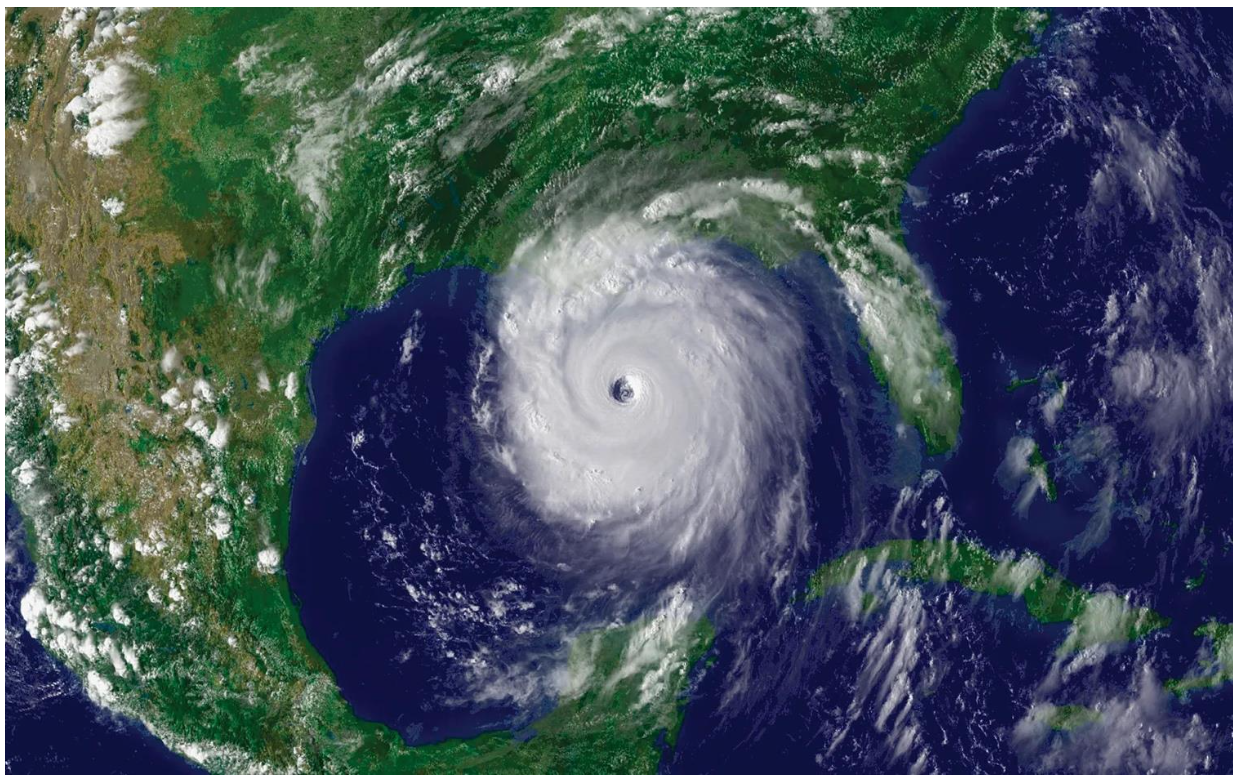
\includegraphics{./figs/hurricane.png}}
%  \end{center}
%  \caption[]{The viscosity of air is $10^{-1}$ cm$^2$/s. Estimate the
%    Reynolds number of a hurricane.}
%  \label{fig:hurricane}
%\end{figure}

\section{Vorticity equation}

\begin{figure}
  \begin{center}
    \resizebox{\textwidth}{!}{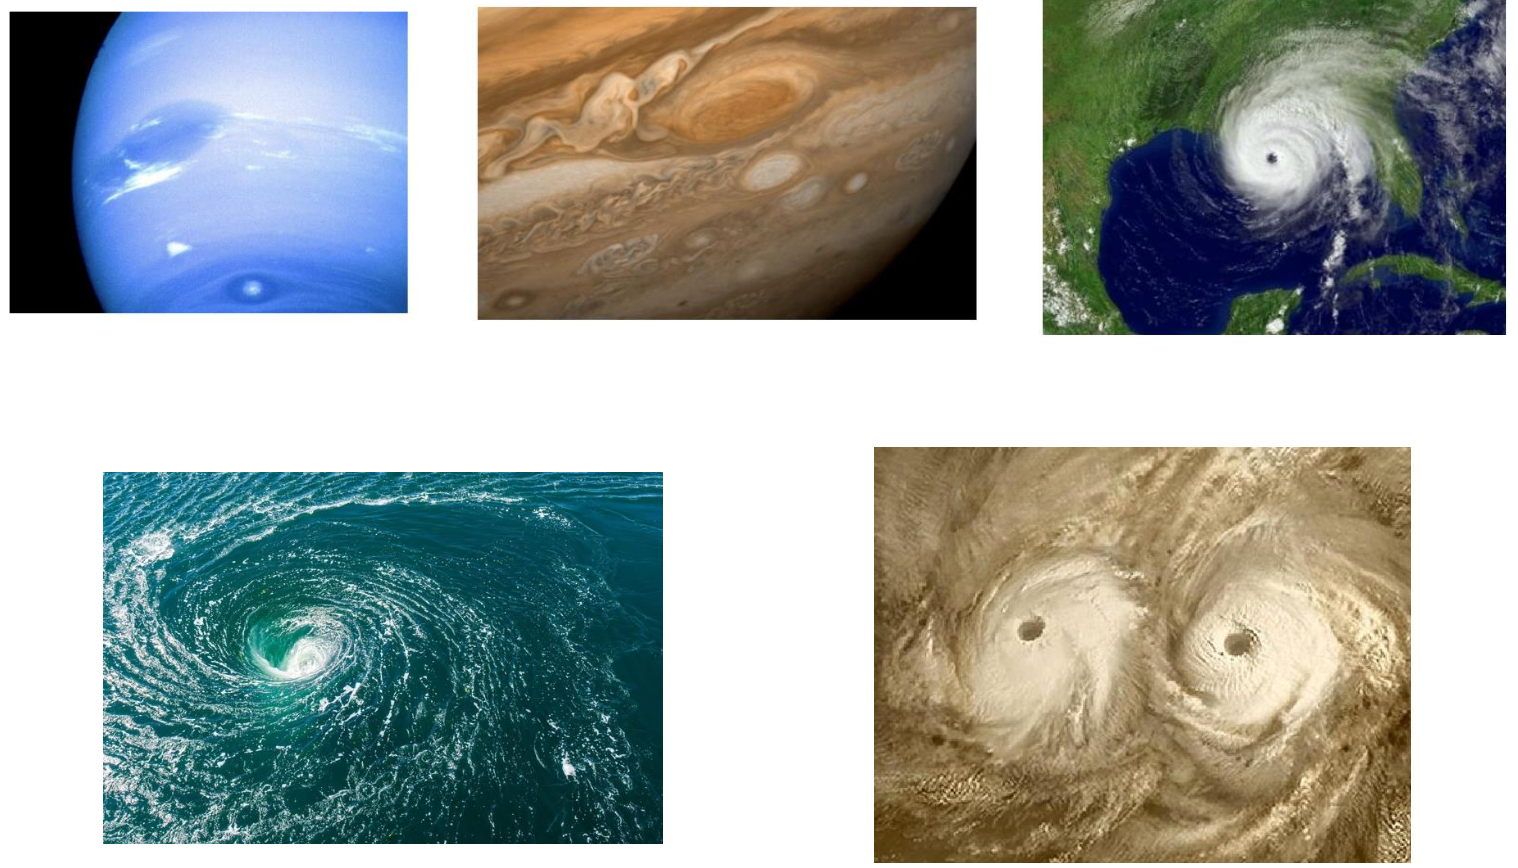
\includegraphics{./figs/vortices.png}}
  \end{center}
  \caption[]{Vortices: an ubiquitous fluid mechanics phenomenon.}
  \label{fig:vortices}
\end{figure}

A view of Jupiter's swirly atmosphere, or following the motion of
hurricanes on Earth, or simply the whirpools in a stream \figp{fig:vortices}, will suffice
to convince you that {\it vortices} are structures that form in flows
and that behave in an independent way than the rest of the
fluid. They're advected by the flow and seem frozen into the fluid as
it flows. 

To understand this behavior, let us define the concept of {\it
  vorticity}. Vorticity is the curl of the velocity

\beq
\v{\omega} = \curl{\v{u}}
\eeq

Indeed, under some conditions (that are often realized in nature), we
will show that vorticity is {\it conserved}. 

If we take the Navier-Stokes equation and curl it

\beq
\frac{\partial \v{\omega}}{\partial t} = -\curl{\left[\left(\v{u}\cdot\del\right)\v{u}\right]}
-\curl{\left(\frac{1}{\rho}\grad{p}\right)} + \curl{\v{f}} + \nu\Laplace\v{\omega}
\eeq

Let us examine the terms. Body forces like gravity are usually conservative, so we set
$\curl{\v{f}}=0$. The curl of the pressure gradient is 

\beq
\curl{\left(\frac{1}{\rho}\grad{p}\right)} =-\frac{1}{\rho^2}\grad{\rho} \times \grad{p}
\eeq

to take the curl of the inertial term we transform 

\beqn
\left(\v{u}\cdot\del\right)\v{u} &=& \frac{1}{2}\grad{u^2} -\v{u}\times\left(\curl{\v{u}}\right)\\
&=&\frac{1}{2}\grad{u^2} -\v{u}\times\v{\omega}
\eeqn

when taking the curl of it, the first term cancels, so we're left with 

\beq
\frac{\partial \v{\omega}}{\partial t} = \curl{\left(\v{u}\times\v{\omega}\right)}
+\frac{1}{\rho^2}\grad{\rho} \times \grad{p} + \nu\Laplace{\v{\omega}}
\label{eq:vort-baro-diff}
\eeq

The curl of the vector product is

\beqn
\curl{\left(\v{u}\times\v{\omega}\right)} &=&\varepsilon_{ijk}\varepsilon_{kpq}\partial_ju_p\omega_q\\
&=&\left(\delta_{ip}\delta_{jq}-\delta_{iq}\delta_{jp}\right)\partial_ju_p\omega_q\\
&=&\partial_ju_i\omega_j - \partial_ju_j\omega_i\\
&=&u_i\partial_j\omega_j +\omega_j\partial_ju_i - u_j\partial_j\omega_i-\omega_i\partial_ju_j\\
&=&\v{u}\left(\Div{\v{\omega}}\right) + \left(\v{\omega}\cdot\del\right) \v{u} -\left(\v{u}\cdot\del\right)\v{\omega} -  \v{\omega}\left(\Div{\v{u}}\right)
\eeqn

Since vorticity is a curl, the first time cancels. What is left yields
the vorticity equation 

\beq
\boxed{
\frac{\partial \v{\omega}}{\partial t} =
-\left(\v{u}\cdot\del\right)\v{\omega}  -
\v{\omega}\left(\Div{\v{u}}\right) + \left(\v{\omega}\cdot\del\right) \v{u} 
+\frac{1}{\rho^2}\grad{\rho} \times \grad{p} + \nu\Laplace{\v{\omega}}
}
\eeq

Let us understand this equation. The first term in the RHS is an
advection term. The second is a compression term. The 3rd term is
stretching, the fourth is the only source term, the baroclinic
term. The last one is diffusion. 

The advection shows that vorticity is advected by the flow, like the
other quantities, so we can write a Langrangian formulation

\beq
\frac{D \v{\omega}}{D t} =- \v{\omega}\left(\Div{\v{u}}\right) +
\left(\v{\omega}\cdot\del\right) \v{u}  +\frac{1}{\rho^2}\grad{\rho} \times \grad{p} + \nu\Laplace{\v{\omega}}
\eeq

The compression term shows that a vortex is amplified if the
flow is compressed, and weakened if the flow expands. Since vorticity
is the fluid circulation, we expect that this is a result of
conservation of angular momentum. 

\subsubsection{The baroclinic term}

A barotropic fluid has $p = p(\rho)$. The surfaces of constant
pressure and constant density are aligned, so the
gradients point in the same direction.
The word barotropic comes from baro (pressure) + tropos
(direction). Meaning pressure gradient is in the same
direction as the density gradient.

A baroclinic fluid has $p = p(\rho,T)$. The surfaces of constant
pressure and constant density can be inclined, with the
gradients pointing in different directions.
The word baroclinic comes from baro (pressure) +
inclination (direction). Meaning pressure and density
gradients are misaligned.

Notice that the polytropic equation of state $p = K \rho^\gamma$ is barotropic.
The interior of stars and giant planets are well-approximated by
polytropes. Notice also that $K=p/\rho^\gamma$ is the entropy. This
means that for barotropic fluids, the entropy is constant.
The condition of baroclinicity then translates simply into: {\it varying entropy}.
An entropy gradient leads to vortex generation by convection \figp{fig:baroclinic}.


\begin{figure}
  \begin{center}
    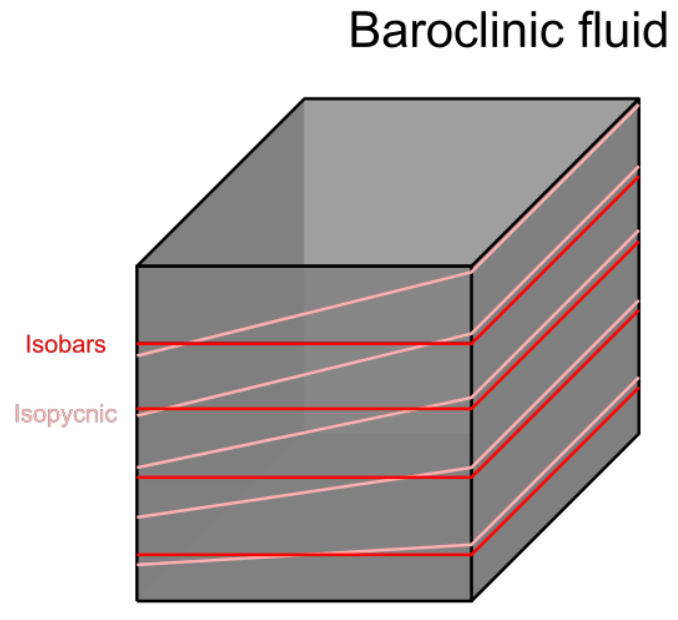
\includegraphics[height=.45\linewidth]{./figs/baroclinicfluid.png}
    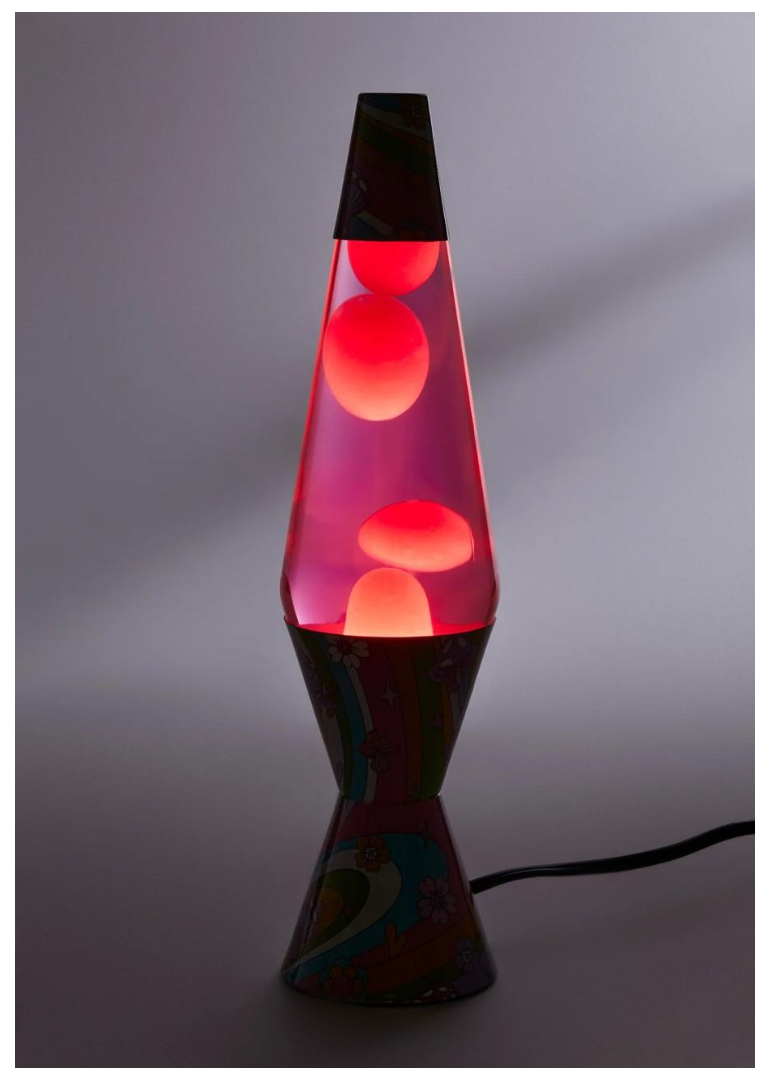
\includegraphics[height=.45\linewidth]{./figs/lavalamp.png} 
%    \resizebox{.47\textwidth}{!}{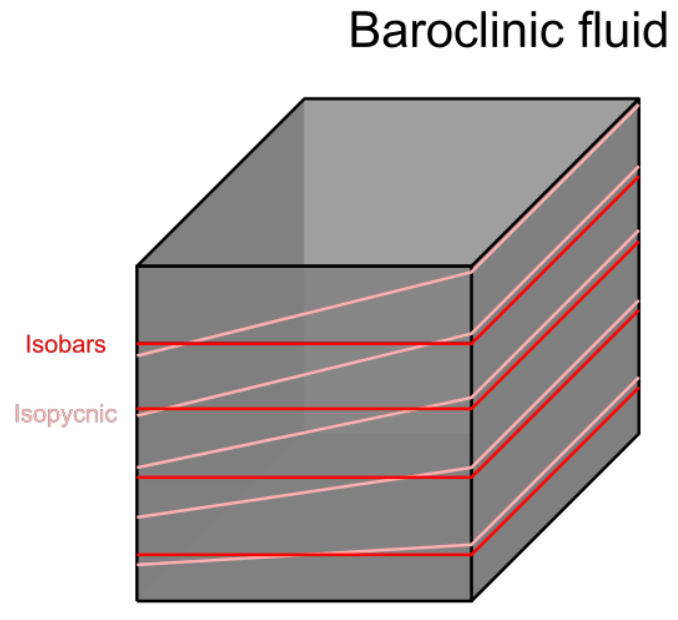
\includegraphics{./figs/baroclinicfluid.png}}
 %   \resizebox{.47\textwidth}{!}{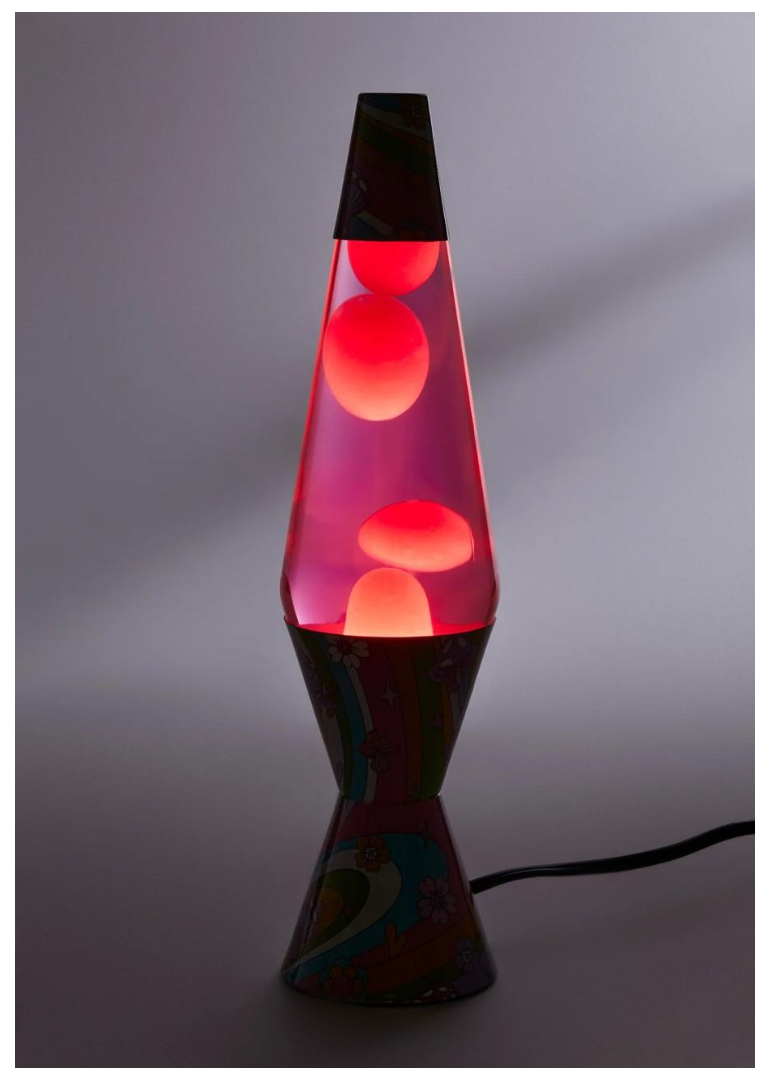
\includegraphics{./figs/lavalamp.png}}
  \end{center}
  \caption[]{Baroclinic fluids: inclined surfaces of constant density
    and constant pressure, i.e., a non-zero
    $\grad{p}\times\grad{\rho}$ is the source of
    vorticity. Alternatively, one can thing of an entropy gradient
    sourcing vorticity, as in convection in a lava lamp.}
  \label{fig:baroclinic}
\end{figure}


\subsubsection{The stretching term}

Let's verify what the strectching term does and why it is called
so. Consider the flow in \fig{fig:stretching}. The velocity points
only in the x-direction, but with a gradient in the y-direction, i.e.,
it has shear. As as
result, it will advect the y-pointing vorticity bundle in a {\it differential}
way. The vorticity at a time in the future will be pointing
diagonally. We started with a vorticity purely in the y-direction, but
a component was built in the x-direction, the direction of the
flow. It was {\it stretched} in the direction of the sheared
flow. Stretching is essentially a sheared advection, changing the
shape of the function, something the advection alone cannot do. It
stretches the vorticity $\v{\omega}$ when the velocity is shearing
in the direction parallel to $\v{\omega}$. Hence its form
$\left(\v{\omega}\cdot\del\right) \v{u}$. 

\begin{figure}
  \begin{center}
    \resizebox{\textwidth}{!}{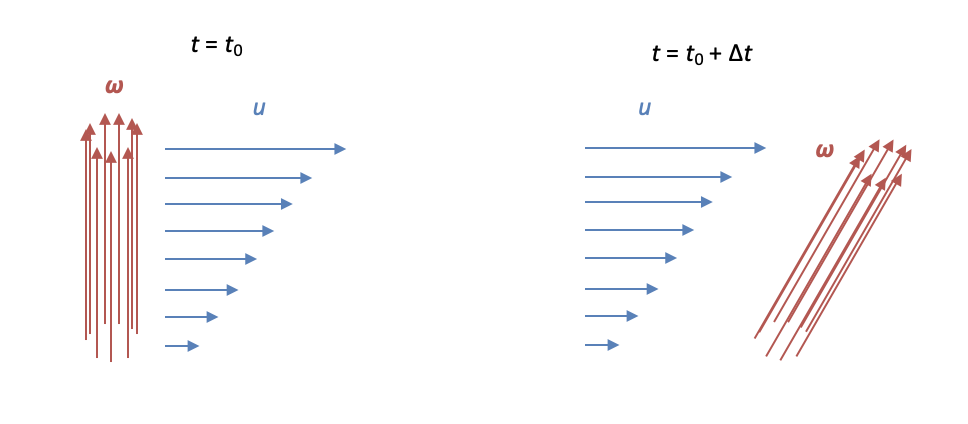
\includegraphics{./figs/stretching.jpg}}
  \end{center}
  \caption[]{Vorticity is amplified in the direction of shear. The
    term responsible for this behavior is the stretching term $\left(\v{\omega}\cdot\del\right)\v{u}$.}
  \label{fig:stretching}
\end{figure}

Notice that if the flow is 2D, there is no stretching, as the
vorticity is perpendicular to the flow, canceling
$\omega_j\partial_j$ \figp{fig:stretching2D}. If on top of that we consider that the flow is
imcompressible, of high Reynolds number, and ignore the baroclinic
term, then vorticity is conserved. 

\beq
\frac{D \v{\omega}}{D t}=0 
\eeq

That vorticity is conserved in this flow explains why vortices are
persistent structures. 

\begin{figure}
  \begin{center}
    \resizebox{.6\textwidth}{!}{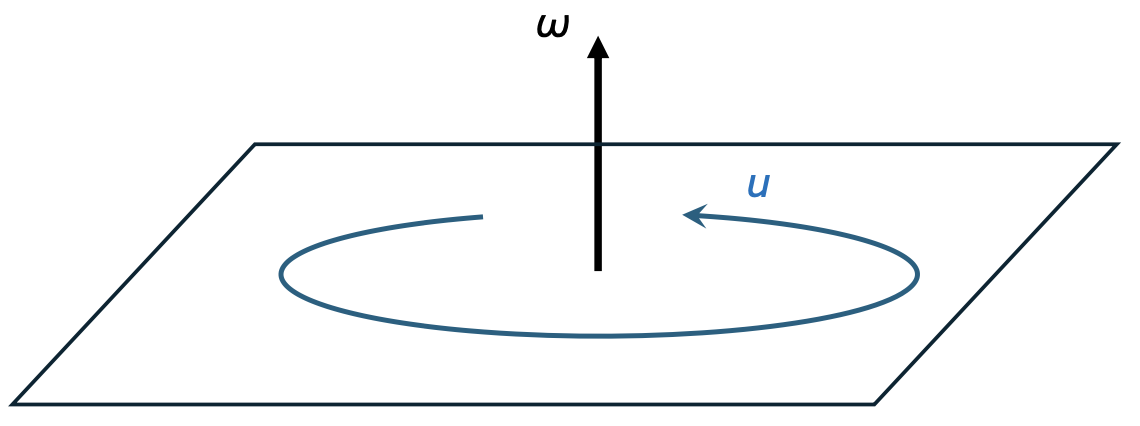
\includegraphics{./figs/stretching2D.png}}
  \end{center}
  \caption[]{If the motion is restricted to a plane, then the
    vorticity is always out of the plane, and the stretching term is zero.}
  \label{fig:stretching2D}
\end{figure}

\section{Kelvin vorticity theorem} 

%VonKarmanStreet.png
%DalembertParadox.png

\begin{figure}
  \begin{center}
    \resizebox{\textwidth}{!}{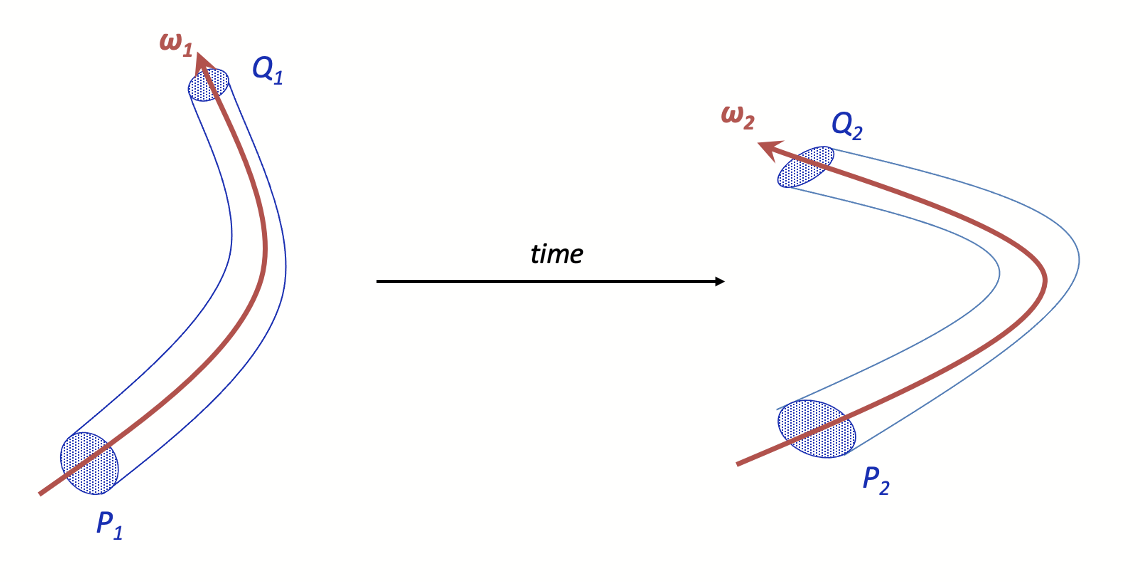
\includegraphics{./figs/KelvinFluxFreezing.png}}
  \end{center}
  \caption[]{Kelvin flux-freezing theorem. Two patches connected by a
    vortex line will remain connected by the same vortex line at
  all times. Irrespective of advection, stretching, and compression,
  the topology of a vortex line is conserved. The vortex is ``frozen''
  on the fluid.}
  \label{fig:KelvinFluxFreezing}
\end{figure}


\begin{figure}
  \begin{center}
    \resizebox{.75\textwidth}{!}{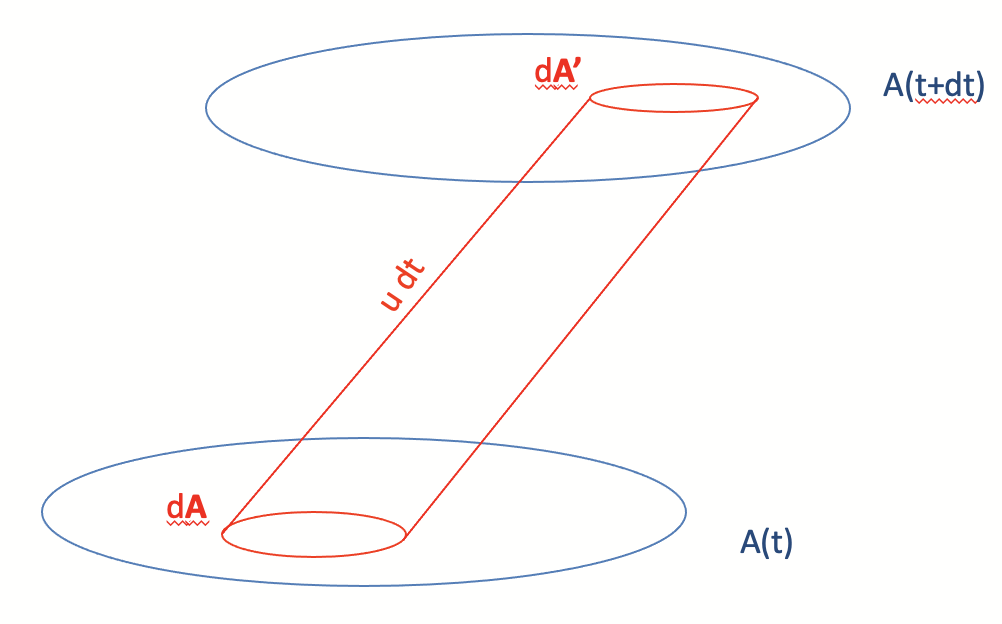
\includegraphics{./figs/KelvinTheorem_Cylinder.png}}
  \end{center}
  \caption[]{A patch $d\v{A}$ flows with velocity $\v{u}$ and is deformed into $d\v{A}^\prime$ within
    a time interval $dt$. This describes a cylinder as given above.}
  \label{fig:KelvinTheorem_Cylinder}
\end{figure}

According to \eq{eq:vort-baro-diff}, a barotropic flow at high
Reynolds numbers satisfies

\beq
\frac{\partial \v{\omega}}{\partial t} = \curl{\left(\v{u}\times\v{\omega}\right)}
\eeq

This equation implies that the flux of vorticity is conserved, and the
vortex lines move with the fluid. This is why we can visualize the
vortices as entities embedded in the fluid:  the vortex lines are ``frozen'' into the
fluid, and move with the flow. This is known as {\it Kelvin's vorticity
theorem} or Kelvin's {\it flux-freezing} theorem. 

The theorem states that

\beq
\frac{d}{dt}\int_A \v{\omega} \cdot d\v{A}  = 0 
\eeq

in plain words, in means that if you consider a surface $A$ inside a
fluid at a given time, the flux of vorticity through this surface is
unchanged as the surface evolves due to whatever motion happens in the fluid.

The consequences of this theorem are remarkable. Once two surface
elements are connected by a vortex line, they will remain so. The
vortex is frozen-in and moves with the fluid \figp{fig:KelvinFluxFreezing}. 

The surface elements $P$ and $Q$ change into $P^\prime$ and $Q^\prime$ as a
result of fluid motions. Due to flux-freezing, the vortex line that
connects $P$ and $Q$ will also connect $P^\prime$ and $Q^\prime$ and
the vortex topology is preserved. This gives a neat visualization of
the vortices: as we can guess the vorticity configuration if we know the
fluid flow. The vortex is an almost material, plastic substance that
moves with the flow. 

Proof:

Kelvin's theorem applies to any vector that satisfies

\beq
\frac{\partial \v{Q}}{\partial t} = \curl{\left(\v{u}\times\v{Q}\right)}
\label{eq:kelvin1}
\eeq

to show that, we need to show that \eq{eq:kelvin1} is equivalent to 

\beq
\frac{d}{dt}\int_A \v{Q} \cdot d\v{A}  = 0 
\eeq

we apply Leibniz rule of derivating under the integral to 

\beq
\frac{d}{dt}\int_A \v{Q} \cdot d\v{A} = \int \frac{\partial
  \v{Q}}{\partial t} dA + \v{Q}\cdot\frac{d}{dt}\left(d\v{A}\right)
\label{eq:kelvin-leib}
\eeq

the term $\frac{d}{dt}\left(d\v{A}\right)$ is the time variation of
a surface element $d\v{A}$. The area $A$ in time $t$ goes to $A^\prime$
in time $t+dt$ \figp{fig:KelvinTheorem_Cylinder}. 


\beq
\frac{d}{dt}\left(d\v{A}\right)  = {\rm lim}_{\Delta t\rightarrow 0}
\frac{d\v{A}^\prime - d\v{A}}{\Delta t}
\eeq

how do we find $d\v{A}^\prime - d\v{A}$?

The vector area integral over a closed surface is zero: $\oint d\v{A}
= 0$. \classcomm{give cube as example}. So let's close the surface  \figp{fig:KelvinTheorem_Cylinder}

The side area is $dS = \oint dl \times \v{u}dt$, so the total area of the
cylinder is

\beq
d\v{A}^\prime -d\v{A} + \oint dl \times \v{u}dt = 0
\eeq

reversing the cross product 

\beq
d\v{A}^\prime -d\v{A} = dt\oint \v{u} \times dl = 0
\eeq

it then follows that

\beq
\frac{d}{dt}\left(d\v{A}\right)  = {\rm lim}_{\Delta t\rightarrow 0}
\frac{d\v{A}^\prime - d\v{A}}{\Delta t} = \oint \v{u} \times dl
\eeq

So the last term of \eq{eq:kelvin-leib} is

\beq
\int_A \v{Q}\cdot \frac{d}{dt}\left(d\v{A}\right) = \int_A \oint \v{Q}\cdot\left(\v{u} \times dl\right)
\eeq

and because 

\beq
\v{A} \cdot \left(\v{B} \times \v{C}\right) = \v{B} \cdot \left(\v{C} \times \v{A} \right)= \v{C} \cdot \left(\v{A} \times \v{B}\right)
\eeq

we can write 

\beq
\int_A \v{Q}\cdot \frac{d}{dt}\left(d\v{A}\right) = \int_A \oint \left(\v{Q}\times\v{u} \right)\cdot dl
\eeq

This is a strange integral. It represents the sum over all little
$d\v{l}$ elements that are 
embedded in the area A. We need to do the line integrals over all the
surface elements that compose A. Because the internal line integrals
cancel out \classcomm{show example of honeycomb pattern} this reduces
to an integral over the contour C of S.

\beq
\int_A \oint \left(\v{Q}\times\v{u} \right)\cdot dl = \oint_C
\left(\v{Q}\times\v{u} \right) dl 
\eeq

which, by Stokes theorem, is

\beq
\oint_C \left(\v{Q}\times\v{u} \right) dl =\int_S
\curl{\left(\v{Q}\times\v{u} \right)} dA
\eeq


So 


\beq
\int_A \v{Q}\cdot \frac{d}{dt}\left(d\v{A}\right) = -\int_S\curl{\left(\v{Q}\times\v{u} \right)} d\v{A}
\eeq

which leads to

\beq
\frac{d}{dt}\int_A \v{Q} \cdot d\v{A}  = \int_A \left[ \frac{\partial    \v{Q}}{\partial t}-\curl{\left(\v{Q}\times\v{u} \right)}\right]
  \cdot d\v{A} 
\eeq

When $\v{Q}$ is vorticity, by the vorticity equation the RHS
cancels. Hence the theorem is proved.

Lord Kelvin, who proved this theorem, was so intrigued
by the permanence of vortices that he even attempted to build a
theory of matter by suggesting that atoms are vortices in the ether. 
One of the strong predictions of Kelvin's theorem is that an ideal fluid
having no vortices at an instant of time cannot subsequently develop
vortices. This could have been inferred from the vorticity equation
itself. Barcolinicity and viscosity make the generation and decay of
vortices possible. A fluid without viscosity would not behave the way
we expect real fluids to behave. When water is splashed against a solid
surface, lots of swirling motions are produced. If a fluid were really
ideal and vortices could not be generated, then such swirling motions
would not take place.


\subsection{D'Alembert's paradox}

\begin{figure}
  \begin{center}
    \resizebox{.75\textwidth}{!}{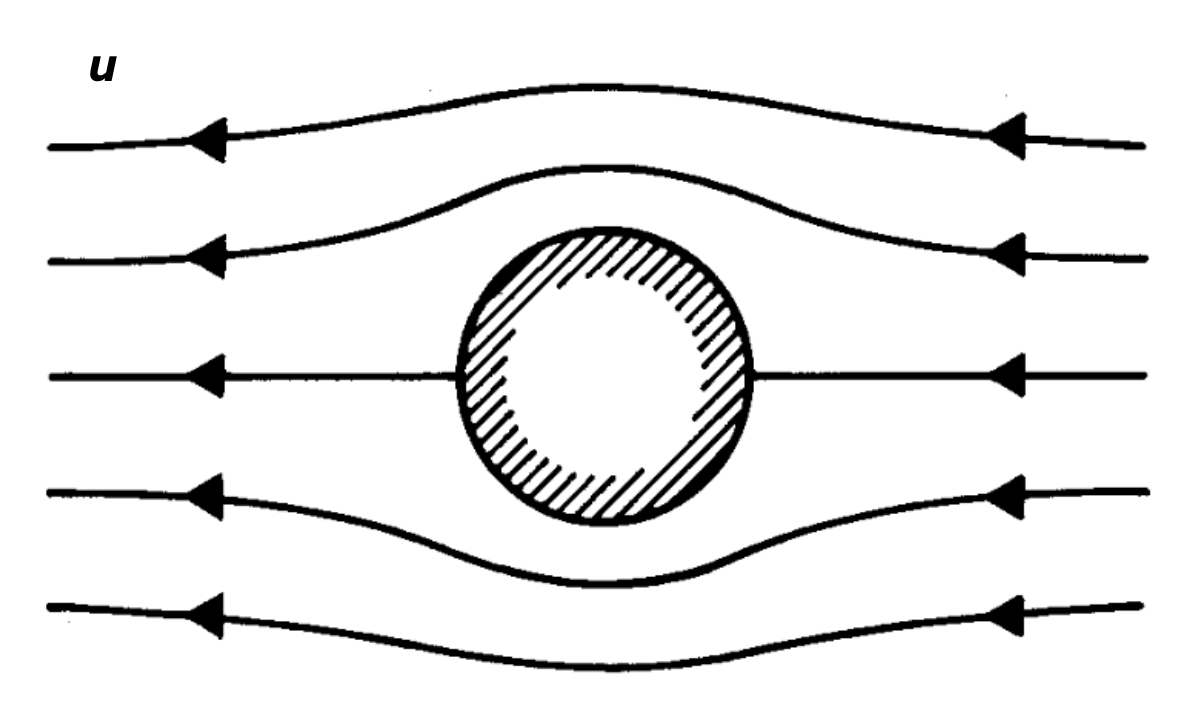
\includegraphics{./figs/DalembertParadox.png}}
  \end{center}
  \caption[]{D'Alembert paradox: a solid moving through an ideal fluid will
    experience no drag, contrary to everyday experience.}
  \label{fig:DalembertParadox}
\end{figure}

Let us find the force on cylinder moving through a
fluid at rest \figp{fig:DalembertParadox}. This is equivalent to a flow past an obstacle at
rest. The obstacle displaces an equal volume of fluid, of mass
$m$. This mass is flowing with velocity u, so its kinetic energy is
$mu^2/2$. The work done by the fluid on the obstable is the time
derivative of the kinetic energy 

\beq
\v{f}\cdot\v{u} =  \frac{dK}{dt} = \frac{m}{2}\frac{d}{dt}\v{u}\cdot\v{u} = m\v{u}\cdot\frac{d\v{u}}{dt}
\eeq

finding the force 

\beq
\v{f} = m\frac{d\v{u}}{dt}
\eeq

This is a curious result. In steady state, there is no force acting on the obstacle. This
goes against our everyday experience that a fluid exerts a drag
force on any object moving through it. This is $d'Alembert's
paradox$, established in 1752. 

This paradox arises because we have neglected viscosity in
our equations. If a body moving through a fluid were to be slowed
by a drag force, the kinetic energy lost in the slowing process has to
go somewhere. In a viscous fluid, it can go to heat. Since this is not
possible in an ideal fluid, we come up with the result that an ideal fluid
cannot exert drag on objects moving through it.

But we have considered that the flow has high Reynolds number. We can
ignore viscosity. What is the problem? 

\subsubsection{Boundary layers}

The solution to the paradox was found by Prandtl in 1904, a century after
D'Alembert established it.

\begin{figure}
  \begin{center}
    \resizebox{\textwidth}{!}{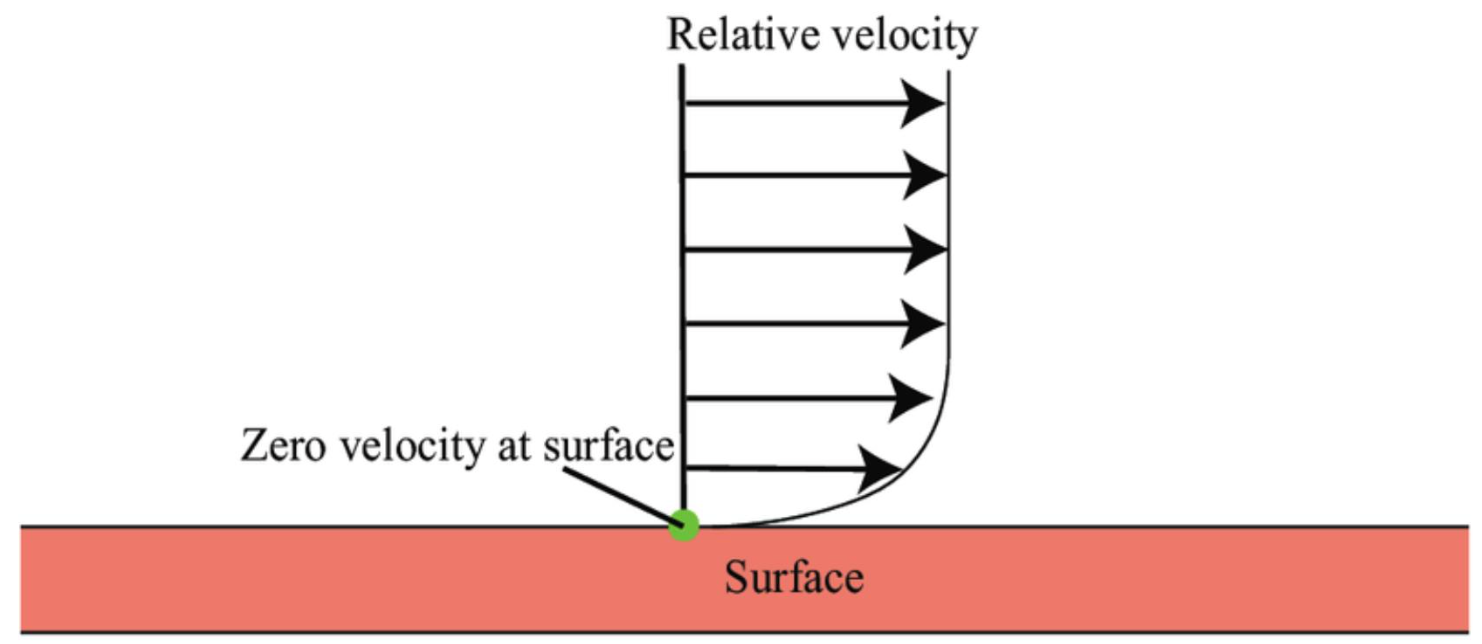
\includegraphics{./figs/noslip_condition.png}}
  \end{center}
  \caption[]{No-slip boundary condition: a fluid comes to rest at a surface.}
  \label{fig:noslip}
\end{figure}

The fluid at the boundary has zero velocity -- which is known as the {\it no-slip boundary
  condition} \figp{fig:noslip}. This leads to strong shear between the boundary at zero,
and the rest of the (moving) fluid. In this region, the shear makes
$\Laplace{\v{u}}$ so strong that viscosity cannot be ignored, even at high
Reynolds number. Essentially, the no-slip boundary condition becomes a
source of vorticity. The viscous term then diffuses the vortex into
the flow. 

\classcomm{Everyday observational experience: the seeing is produced inside the dome.}

Consider pipe flow. The flow is established by a pressure gradient,
and in equilibrium with the viscous force

\beq
\mu\Laplace{\v{u}}=\grad{p} 
\eeq

\noindent approximating $\grad{p}=\Delta p / L$ where $L$ is the length of the
pipe, and writing $\Laplace{\v{u}}$ in cylindrical coordinates 

\beq
\frac{1}{r}\frac{d}{dr}\left(r\frac{du}{dr}\right) =\frac{\Delta p}{\mu L} 
\eeq

\noindent with boundary conditions $u=0$ at $r=a$ (no slip condition), and
$du/dr=0$ at $r=0$ (so the flow is continuous).

\beq
\frac{d}{dr}\left(r\frac{du}{dr}\right) =\frac{\Delta p}{\mu L} r
\eeq

\noindent and integrating 

\beq
r\frac{du}{dr} =\frac{\Delta p}{2\mu L} r^2 + C_1
\eeq

\noindent dividing by $r$

\beq
\frac{du}{dr} =\frac{\Delta p}{2\mu L} r + \frac{C_1}{r}
\eeq

\noindent the Newman boundary condition at $r=0$ implies $C_1=0$. Integrating again

\beq
u(r) =\frac{\Delta p}{4\mu L} r^2 + C_2 
\eeq

\noindent and the Dirichlet boundary condition $u=0$ at $r=a$, implies 

\beq
u(r) =\frac{\Delta p}{4\mu L} \left(r^2 -a^2\right)
\eeq

\noindent so the flow is parabolic \figp{fig:pipe_flow}.

\begin{figure}
  \begin{center}
    \resizebox{\textwidth}{!}{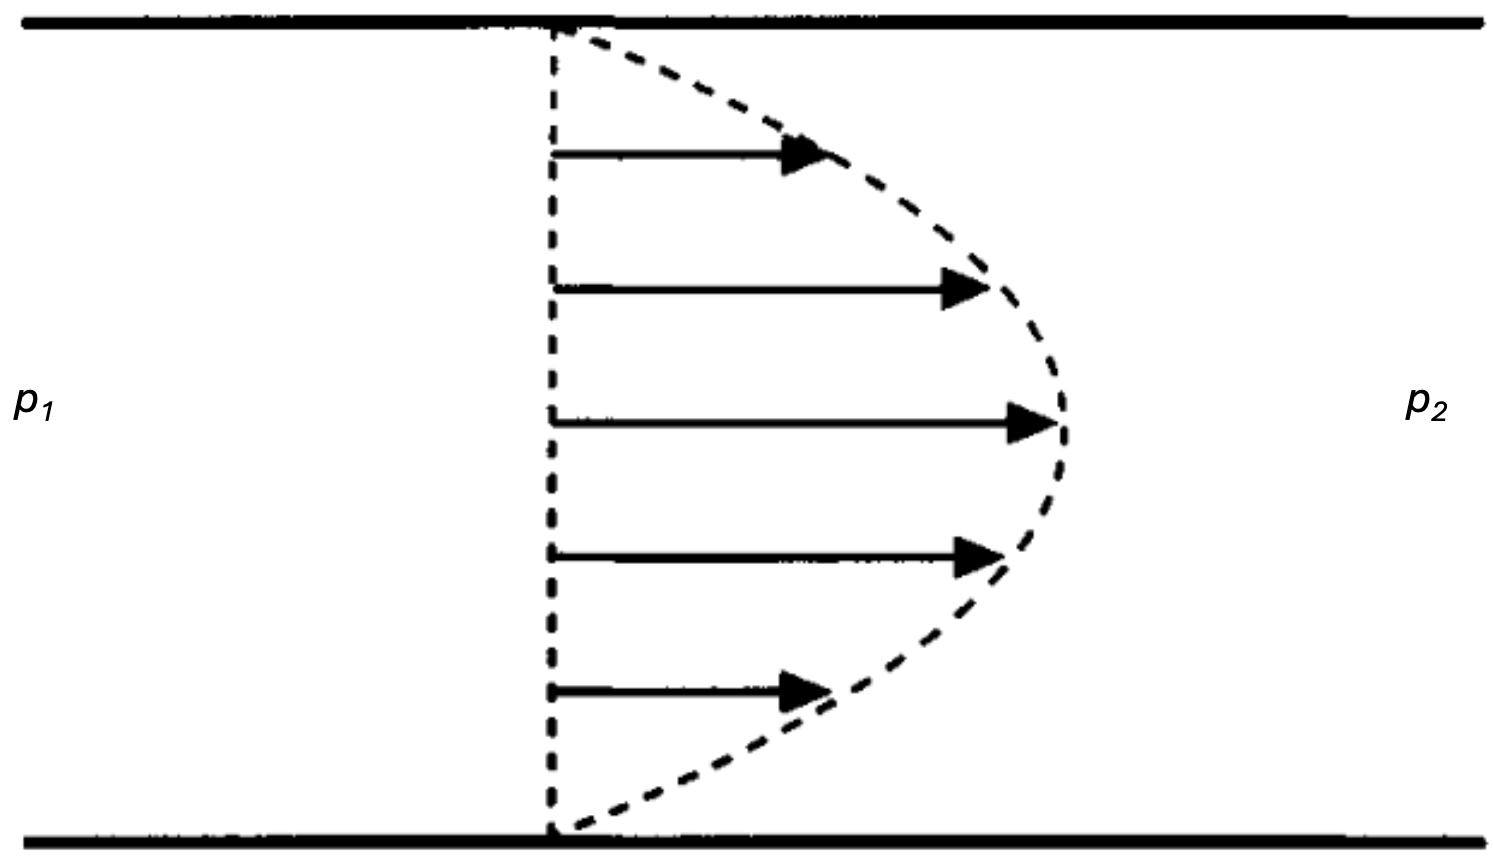
\includegraphics{./figs/pipe_flow.png}}
  \end{center}
  \caption[]{Pipe flow. The flow comes to rest at the boundary,
    assuming a parabolic shape.}
  \label{fig:pipe_flow}
\end{figure}


\subsection{Shear and flow past an obstacle}

Notice that this flow has vorticity. 

\beq
\omega = \frac{\partial u_x}{\partial y}
\eeq

A viscous flow can start with zero shear, and the no-slip
condition develops shear and vorticity. This is an important
qualitative concept to internalize: {\it a boundary is a vorticity
  source}. This is clearly illustrated in the von Karman vortex
street, one of the most beautiful phenomena of fluid dynamics
\figp{fig:vonkarman}. Past the obstacle, the flow develops vortices of
opposite polarity in the flow downstream. 

\begin{figure}
  \begin{center}
    \resizebox{\textwidth}{!}{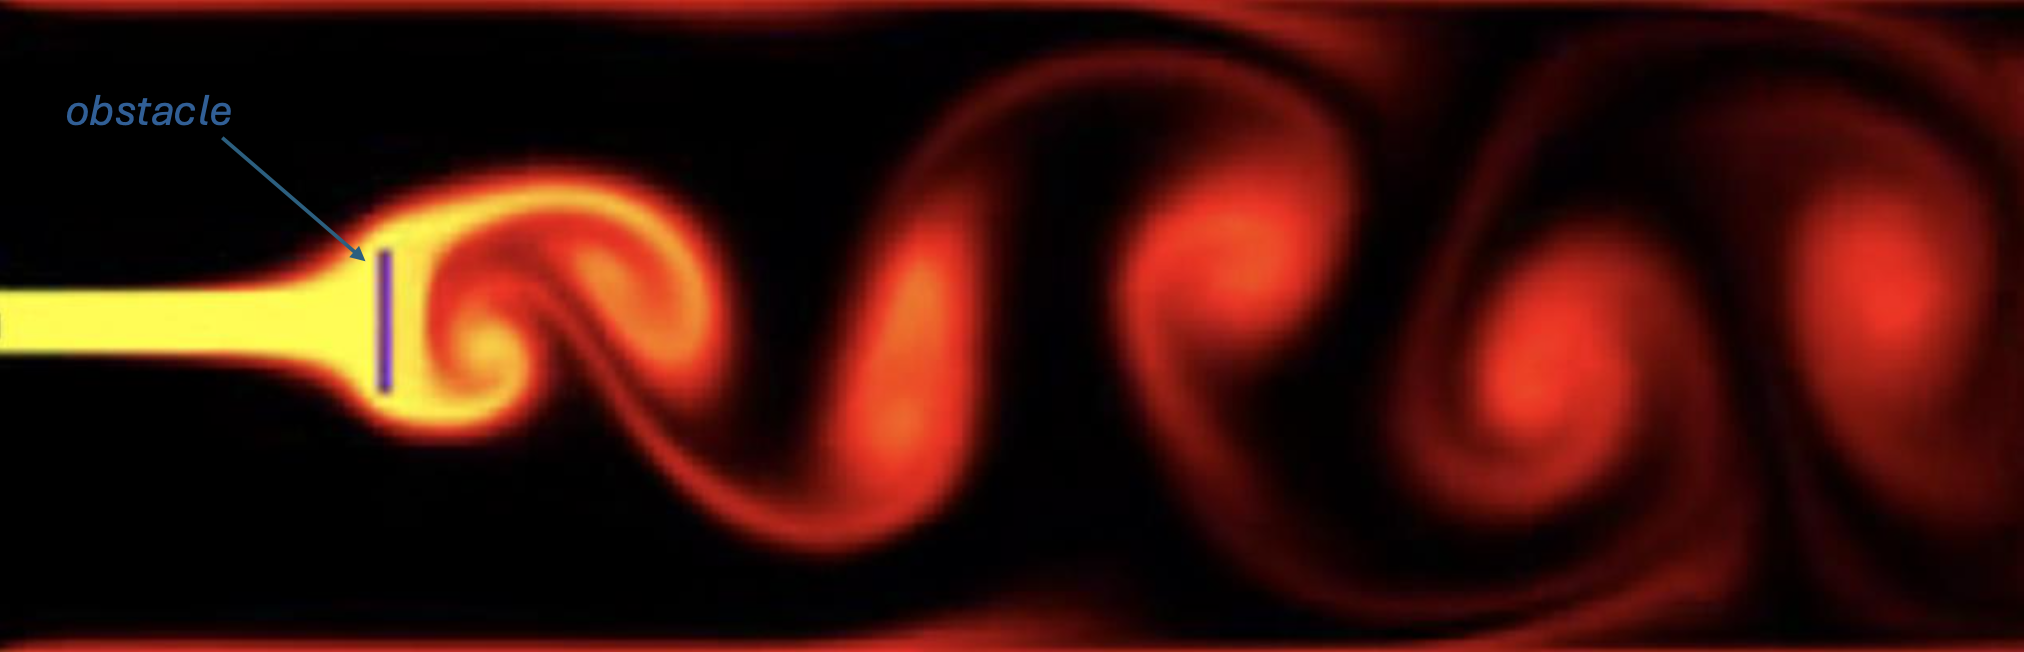
\includegraphics{./figs/VonKarmanStreet.png}}
  \end{center}
  \caption[]{von Karman vortex street in flow past an obstacle.}
  \label{fig:vonkarman}
\end{figure}

But how is the shear developed at the boundary layer converted into
vorticity? We will tackle that when studying Kelvin-Helmholtz and
Rayleigh-Taylor instabilities. For now, let us notice that {\it shear and
vorticity have the same dimension}. The definition of the shear tensor is

\beq
S_{ij} = \frac{1}{2}\frac{\partial u_i}{\partial x_j} + \frac{\partial u_j}{\partial x_i} 
\eeq

\noindent whereas the rotation tensor is 

\beq
\Omega_{ij} = \frac{1}{2}\frac{\partial u_i}{\partial x_j} - \frac{\partial u_j}{\partial x_i} 
\eeq

The vorticity is defined as

\beq
\Omega_{ij}=-\frac{1}{2}\varepsilon_{ijk}\omega_k
\eeq

\noindent shear and vorticity are two sides of the same coin. 

\section{Rotating frames}


\begin{figure}
  \begin{center}
    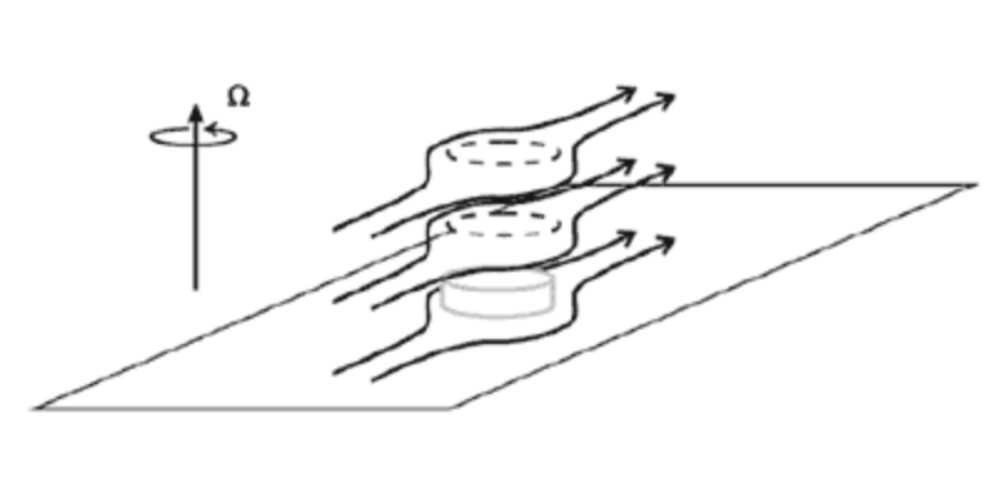
\includegraphics[height=.35\linewidth]{./figs/tp1.png}
    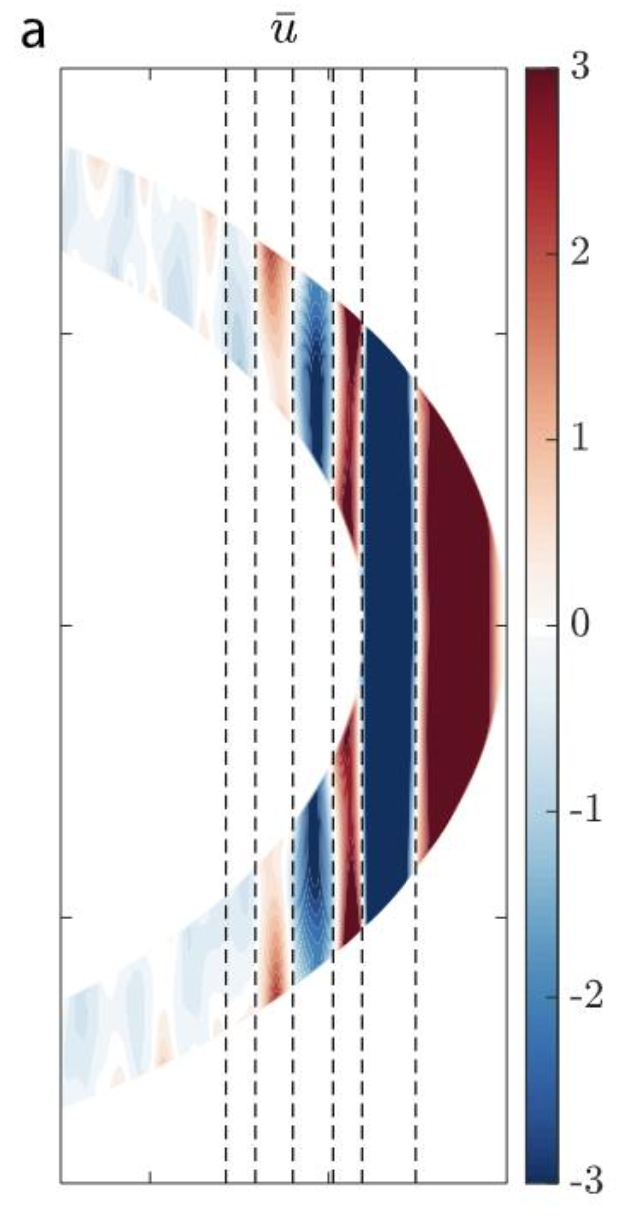
\includegraphics[height=.45\linewidth]{./figs/tp2.png} 
  \end{center}
  \caption[]{Left: The Taylor-Proudmann theorem demands that vertical
    columns of fluid move along contours of constant fluid depth. Thus
    fluid columns act as if they were rigid and move along contours of
    constant fluid depth. Horizontal flow is thus deflected as if the
    obstacle extedned through the whole depth of the fluid. Right:
    Interior model of Jupiter showing how a fast rotator shows a flow
    pattern constant in cylinders along the rotation axis.}
  \label{fig:taylor-proudmann}
\end{figure}

\classcomm{show vortex street over Madeira}

In astrophysics it is often useful to work in a frame rotating with constant
angular speed $\v{\Omega}$. This may be the frame in which a binary system is
stationary, a rotating fluid is at rest, or a spiral pattern is stationary. In
a rotating frame, we simply add the Coriolis and centrifugal forces to
the RHS of the Euler equation, which gives the forces acting on fluid
elements, just as we would do for Newtonian point-particle mechanics.
Thus the Euler equation in a rotating frame is

\beq
\ptderiv{\v{u}} +\left(\v{u}\cdot  \grad\right) \v{u} =
-\frac{1}{\rho}\grad{p}  - 2\v{\Omega}\times\v{u} - \v{\Omega}\times\v{\Omega}\times\v{r}
\eeq

and the velocity measured in the inertial frame is

\beq
\v{u}_{\rm inertial} = \v{u} + \v{\Omega}\times\v{r}
\eeq

\subsection{Taylor-Proudman theorem}

If the centrifugal force can be neglected, a steady state flow will be
in equilibrium between the pressure gradient and the Coriolis
force. Such a flow is called {\it geostrophic} flow

\beq
2\v{\Omega}\times\v{u} = -\frac{1}{\rho}\grad{p} 
\eeq

\noindent taking the curl eliminates the pressure gradient, leading to 

\beq
\curl{\left(\v{\Omega}\times\v{u}\right)}  = 0 
\eeq

\noindent in index notation, the LHS is 

\beqn
\varepsilon_{ijk}\partial_j\varepsilon_{kpq}\Omega_p u_q &=&
\left(\delta_{ip}\delta_{jq}-\delta_{iq}\delta_{jp}\right) \partial_j
\Omega_p u_q\\
&=&\Omega_i\partial_j u_j - \Omega_j\partial_ju_i\\
\eeqn

\noindent where we considered $\v{\Omega}$ to be constant. If the flow is
imcompressible,

\beq
\left(\v{\Omega}\cdot\del\right)\v{u}=0
\eeq

Without loss of generality, we can
choose the axis $z$ to align with $\v{\Omega}$. In this case, the
theorem reduces to

\beq
\frac{\partial\v{u}}{\partial z} = 0 
\eeq

This remarkable theorem says that the flow is constant in cylinders:
symmetric around the rotation axis \figp{fig:taylor-proudmann}.

\classcomm{Show Sun and Jupiter rotation profiles}


\section{Acoustics}

Let us consider the isothermal hydro equations, in the absence of body forces 

\begin{eqnarray}
\frac{\partial \rho}{\partial t}  + \left(\v{u}\cdot \nabla\right)\rho  &=& -\rho \nabla \cdot \v{u}   \\
\frac{\partial \v{u}}{\partial t}  +  \left(\v{u}\cdot \nabla\right) \v{u} &=& -\frac{1}{\rho} \nabla p 
\end{eqnarray}

%and closed with the equation of state for ideal gases

%\begin{equation}
%p = \rho c_s^2/\gamma
%\end{equation}

%with $\gamma=1$ for isothermal and $c_s$ is the sound speed

And consider a one-dimensional configuration, so that $\v{u}=u$

\begin{eqnarray}
\frac{\partial \rho}{\partial t}  + u\frac{\partial \rho}{\partial x} &=& -\rho\frac{\partial u}{\partial x}    \\
\frac{\partial u}{\partial t}  +  u\frac{\partial u}{\partial x} &=& -\frac{1}{\rho} \frac{\partial p}{\partial x}  \\
\end{eqnarray}

This system admits waves. To find the waves, let us linearize the system, decomposing it into base and perturbation, ie any quantity $Q$ is decomposed into a base state $\bar{Q}$ and a perturbation $Q^\prime$

\begin{equation}
Q = \bar{Q} + Q^\prime
\end{equation}

This way, the equations are expressed as  


\begin{eqnarray}
\frac{\partial (\bar{\rho}+\rho^\prime)}{\partial t}  + (\bar{u}+u^\prime)\frac{\partial (\bar{\rho}+\rho^\prime)}{\partial x} &=& -(\bar{\rho}+\rho^\prime)\frac{\partial (\bar{u}+u^\prime)}{\partial x}   \\
\frac{\partial (\bar{u}+u^\prime)}{\partial t}  +  (\bar{u}+u^\prime)\frac{\partial (\bar{u}+u^\prime)}{\partial x} &=& -\frac{1}{(\bar{\rho}+\rho^\prime)} \frac{\partial (\bar{p}+p^\prime)}{\partial x} 
\end{eqnarray}

consider now that the base state is constant, so its derivatives (in time and space) cancel 


\begin{eqnarray}
\frac{\partial \rho^\prime}{\partial t}  + (\bar{u}+u^\prime)\frac{\partial \rho^\prime}{\partial x} &=& -(\bar{\rho}+\rho^\prime)\frac{\partial u^\prime}{\partial x}   \\
\frac{\partial u^\prime}{\partial t}  +  (\bar{u}+u^\prime)\frac{\partial u^\prime}{\partial x} &=& -\frac{1}{(\bar{\rho}+\rho^\prime)} \frac{\partial p^\prime}{\partial x} 
\end{eqnarray}

consider also that the system is Galilean-invariant, so we can set $\bar{u}=0$ 

\begin{eqnarray}
\frac{\partial \rho^\prime}{\partial t}  + u^\prime\frac{\partial \rho^\prime}{\partial x} &=& -(\bar{\rho}+\rho^\prime)\frac{\partial u^\prime}{\partial x}   \\
\frac{\partial u^\prime}{\partial t}  +  u^\prime\frac{\partial u^\prime}{\partial x} &=& -\frac{1}{(\bar{\rho}+\rho^\prime)} \frac{\partial p^\prime}{\partial x} 
\end{eqnarray}

and that the base state of density is much larger than its pertubation $\bar{\rho}\gg \rho^\prime$. 

\begin{eqnarray}
\frac{\partial \rho^\prime}{\partial t}  + u^\prime\frac{\partial \rho^\prime}{\partial x} &=& -\bar{\rho}\frac{\partial u^\prime}{\partial x}   \\
\frac{\partial u^\prime}{\partial t}  +  u^\prime\frac{\partial u^\prime}{\partial x} &=& -\frac{1}{\bar{\rho}} \frac{\partial p^\prime}{\partial x} 
\end{eqnarray}

Two primed quantities are of second order, and ignored, canceling the nonlinear term. We have thus a simple system 

\begin{eqnarray}
\frac{\partial \rho^\prime}{\partial t}   &=& -\bar{\rho}\frac{\partial u^\prime}{\partial x}   \\
\frac{\partial u^\prime}{\partial t}   &=& -\frac{1}{\bar{\rho}} \frac{\partial p^\prime}{\partial x} 
\end{eqnarray}

\section{Wave solution}

We take the time derivative of both equations 


\begin{eqnarray}
\frac{\partial^2 \rho^\prime}{\partial t^2}   &=& -\bar{\rho}\frac{\partial }{\partial x} \frac{\partial u^\prime}{\partial t}  \\
\frac{\partial^2 u^\prime}{\partial t^2}   &=& -\frac{1}{\bar{\rho}} \frac{\partial }{\partial x} \frac{\partial p^\prime}{\partial t} 
\end{eqnarray}

and substituting the equation for the time derivative of $u^\prime$

\begin{eqnarray}
\frac{\partial^2 \rho^\prime}{\partial t^2}   &=& \frac{\partial^2 p^\prime}{\partial x^2} \\
\frac{\partial^2 u^\prime}{\partial t^2}   &=& -\frac{1}{\bar{\rho}} \frac{\partial }{\partial x} \frac{\partial p^\prime}{\partial t} 
\end{eqnarray}


%To progress, we need an equation of state. We will use the ideal gas law, which leads to 

To progress, we consider that the pressure is a function of density,
and write

\beq
\partial p = \partial \rho c_s^2 
\eeq

where

\beq
c_s^2 \equiv \frac{\partial p}{\partial \rho}.
\eeq

Given the dimensions, $c_s$ must have dimension of velocity. As will become clear soon, this is
the sound speed. Making this substitution


\begin{eqnarray}
\frac{\partial^2 \rho^\prime}{\partial t^2}   &=& c_s^2 \frac{\partial^2 \rho^\prime}{\partial x^2} \\
\frac{\partial^2 u^\prime}{\partial t^2}   &=& -\frac{c_s^2}{\bar{\rho}} \frac{\partial }{\partial x} \frac{\partial \rho\prime}{\partial t} 
\end{eqnarray}

substituting the equation for the time derivative of $\rho^\prime$

\begin{eqnarray}
\frac{\partial^2 \rho^\prime}{\partial t^2}   &=& c_s^2 \frac{\partial^2 \rho^\prime}{\partial x^2} \\
\frac{\partial^2 u^\prime}{\partial t^2}   &=& c_s^2 \frac{\partial^2 u^\prime}{\partial x^2}
\end{eqnarray}

These are {\it wave equations}, that describe a sound wave. The speed of the wave is the sound speed $c_s$. The wave propagates in the same direction of travel, being longitudinal. 

\section{Dispersion relation}

Another way to derive the wave solution is by finding the {\it dispersion relation}, which is the relation between frequency and wavelength. Considering again the original equations 

\begin{eqnarray}
\frac{\partial \rho^\prime}{\partial t}   &=& -\bar{\rho}\frac{\partial u^\prime}{\partial x}   \\
\frac{\partial u^\prime}{\partial t}   &=& -\frac{1}{\bar{\rho}} \frac{\partial p^\prime}{\partial x} 
\end{eqnarray}

Let us decompose the fields $\rho$ and $u$ into Fourier modes $\psi = \hat{\psi} \mbox{exp}[-i(\omega t + kx)]$

\begin{eqnarray}
-i\omega\hat{\rho} &=& \bar{\rho} i k \hat{u} \\
-i\omega\hat{u}  &=& \frac{c_s^2}{\bar{\rho}}ik\hat{\rho}  
\end{eqnarray}

Isolating $\hat{u}$ in the second equation and substituting it on the first 

\begin{equation}
\omega^2= k^2 c_s^2 
\end{equation}

so $\omega = \pm k c_s$. Plugging it back in the Fourier mode 

\begin{equation}
\psi = \hat{\psi} \mbox{exp}[-i k ( x + c_s t)]
\end{equation}

The system is Galilean invariant over the transformation $x \longrightarrow x \pm c_s t$, so this is a wave, propagating with velocity $c_s$, the sound speed. 


\section{Shocks}


\subsection{Burgers' equation - Steepening of gradients}

Consider the Euler equation without pressure 

\beq
\frac{\partial \v{u}}{\partial t}  + \left(\v{u}\cdot\del\right)\v{u} = 0 
\eeq

this is known and the inviscid Burgers' equation, and is equivalent to
the advection equation with the velocity itself being advected. In 1D,
this becomes 

\beq
\frac{\partial u}{\partial t}  + u \frac{\partial u}{\partial x} = 0 
\eeq

The solution of this equation leads to distortions and eventually an
infinite gradient, a discontinuity in the flow. This process is called
non-linear ``steepening'' of gradients \fig{fig:steepening}. \classcomm{Show steepening of
  gradient solution}.

As a shock forms, the conservation equations relate the quantities
upstream and downstream across the discontinuity jump. These are the Rankine-Hugonit
jump conditions.

\begin{figure}
  \begin{center}
    \resizebox{\textwidth}{!}{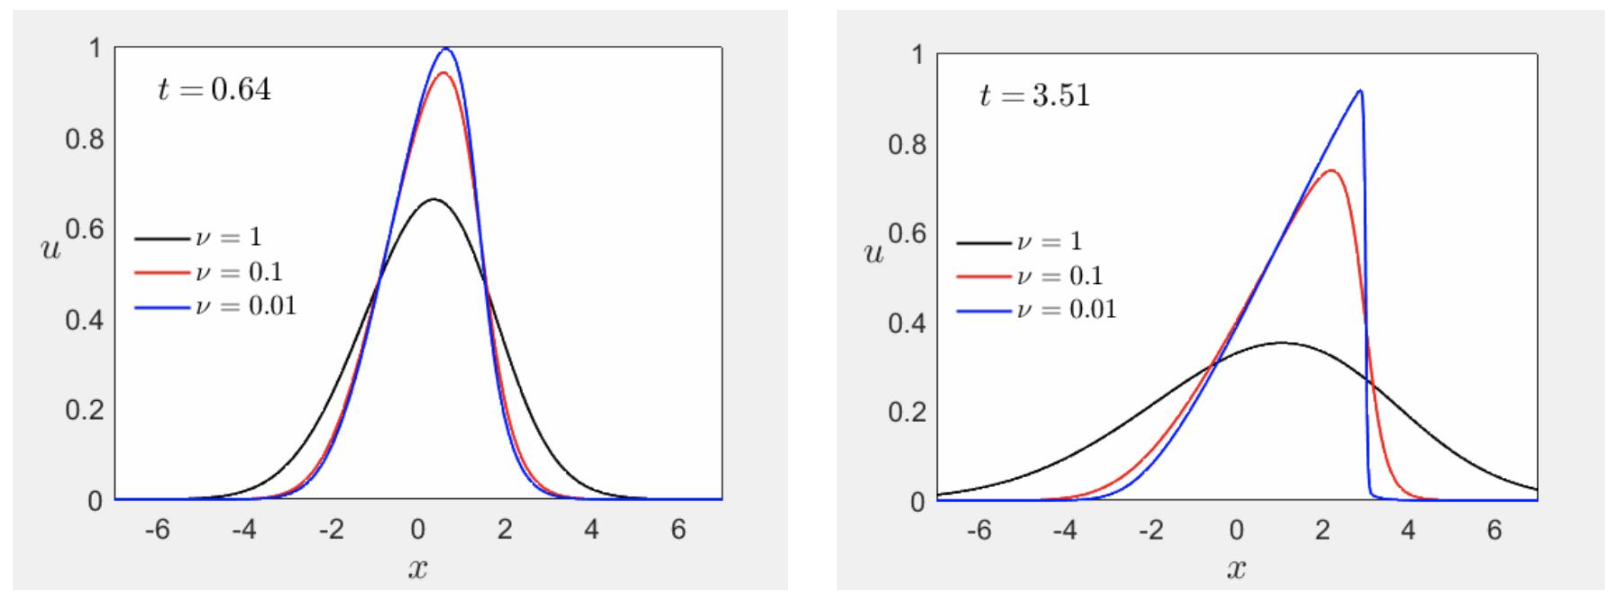
\includegraphics{./figs/steepening.png}}
  \end{center}
  \caption[]{Without sound waves or viscosity, any gradient in the flow
    will steepen and develop a discontinuity.}
  \label{fig:steepening}
\end{figure}


\subsection{Rankine-Hugoniot jump conditions}

To find the jump conditions, let us consider a plane-parallel 1D shock
\figp{fig:parallelshock}. The flow has a discontinuity over which
density, velocity, and pressure change. Yet, the hydro equations must
be obeyed across the jump. Let us consider them in 
conservative form, for mass \eqp{eq:continuity-conservative}, momentum
\eqp{eq:momentum-conservative}, and energy
\eqp{eq:energy-conservative}.  Applying state steady and no external forces these equations yield

\beqn
\Div{\left(\rho\v{u}\right)} &=& 0\\
\Div{ \left(\rho\v{u}\otimes\v{u} + \vt{P}\right)} &=& 0\\
\Div{\left[\left(\frac{u^2}{2}+ e+\frac{p}{\rho}\right)\rho\v{u}\right]} &=&0
\eeqn

in the Euler equation we substituted $\vt{P}=p\vt{I}$, and in the
energy equation $E = \frac{\rho u^2}{2}+\rho e$. These conditions
immediately imply, that across the discontinuity the quantities must
obey 

\begin{figure}
  \begin{center}
    \resizebox{\textwidth}{!}{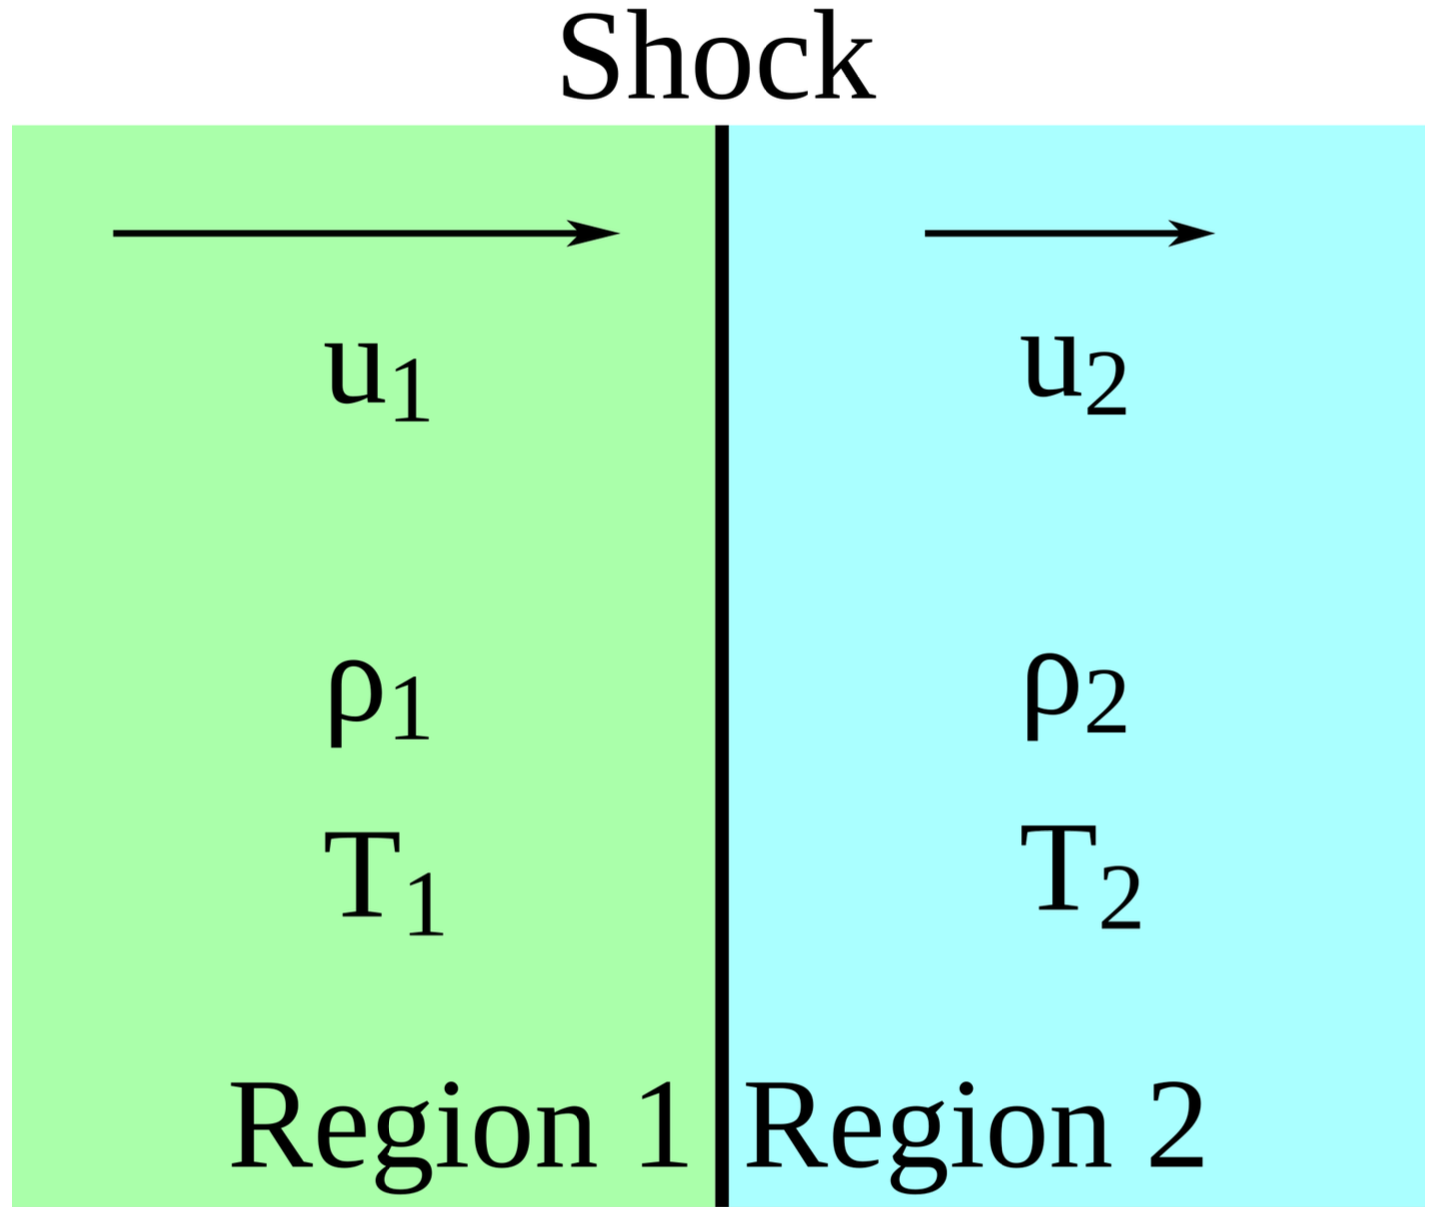
\includegraphics{./figs/parallel_shock.png}}
  \end{center}
  \caption[]{Geometry of a 1D plane-parallel shock. The shock is
    discontinuous, but the flux of mass, momentum, and energy are
    constant, obeying the conservation laws. This allows us to find
    relations between the quantities upstream and downstream, the
    Rankine-Hugoniot jump conditions.}
  \label{fig:parallelshock}
\end{figure}


\beqn
\rho_1 u_1 &=& \rho_2 u_2  \label{eq:rh-mass}\\
\rho_1 u_1^2 + p_1 &=& \rho_2 u_2^2 + p_2 \label{eq:rh-momentum}\\
\frac{1}{2}u_1^2+ e_1 + \frac{p_1}{\rho_1}&=&\frac{1}{2}u_2^2+ e_2 + \frac{p_2}{\rho_2}\label{eq:rh-energy}
\eeqn

The last one because the derivative of $\rho u$ is zero according to
the continuity equation.

30 min of algebra (not to be repeated here) will yield the relations for $\rho$, $u$ and $T$
pre-and-post shock in terms of the Mach number of the flow upstream 

\beqn
\frac{\rho_2}{\rho_1} = \frac{u_2}{u_1} &=& \frac{\left(\gamma+1\right)  \Ma_1^2}{\left(\gamma-1\right) \Ma_1^2+2}\\
\frac{p_2}{p_1} &=& \frac{2\gamma \Ma_1^2 - \left(\gamma-1\right)}{\left(\gamma+1\right)}\\
\frac{T_2}{T_1} &=& \frac{\left[2\gamma \Ma_1^2 - \left(\gamma-1\right)\right]\left[\left(\gamma-1\right)\Ma_1^2+2\right]}{\left(\gamma+1\right)\Ma_1^2}
\eeqn

for a strong shock $\Ma \gg 1$, these become


\beqn
\frac{\rho_2}{\rho_1} = \frac{u_2}{u_1} &=& \frac{\left(\gamma+1\right)}{\left(\gamma-1\right)}\\
p_2 &=& p_1 \ \Ma^2 \ \frac{2\gamma}{\gamma+1}\\
T_2 &=& T_1 \ \Ma^2\ \frac{2\gamma\left(\gamma-1\right)}{\left(\gamma+1\right)^2}
\eeqn

notice how $\rho$ and $u$ do not depend on the Mach number. For
$\gamma=5/3$,  $\frac{\rho_2}{\rho_1} = \frac{u_2}{u_1}=4$.


The temperature 

\beq
T_2 = T_1 \ \Ma^2\
\frac{2\gamma\left(\gamma-1\right)}{\left(\gamma+1\right)^2} =
\frac{m}{k} u_1^2 \frac{2\gamma\left(\gamma-1\right)}{\left(\gamma+1\right)^2}
= \frac{3}{16}\frac{m}{k} u_1^2
\eeq

So the thermal energy postshock is

\beq
\frac{3}{2}\frac{kT_2}{m} = \frac{9}{32} u_1^2
\eeq

compare that to the kinetic energy postshock, which decreased by a
factor 16. 

\beq
\frac{1}{2}u_2^2 = \frac{1}{32}u_1^2 
\eeq

So roughly half of the pre-shock kinetic energy is converted to thermal energy. The total energy
of the post-shock gas is lower (in the shock rest frame) because of the work done on the gas by
viscosity and pressure in the shock.

A shock converts supersonic gas into denser, slower moving, higher pressure, subsonic gas. It
increases the specific entropy of the gas by an amount

\beq
\Delta s = s_2 - s_1 = c_V \left[\ln \left(\frac{P_2}{P_1}\right)
  -\gamma\ln \left(\frac{\rho_2}{\rho_1}\right)\right] > 0
\eeq

What are places where astrophysical shocks occur?

\begin{itemize}
\item Cloud-cloud collisions
\item HII regions expanding into neutral medium
\item Stellar wind encountering medium
\item Supernova or GRB blast wave (internal and external shocks)
\item Accretion onto compact objects: spherical or disk
\item Accretion onto hydrostatic intracluster medium
\end{itemize}

In general a shock wave is
\begin{itemize}
\item a pressure driven compressive disturbance
\item propagating faster than the “signal speed” for compressive waves
\item producing irreversible change in fluid state (increase of entropy)
\end{itemize}



%References: S. Hofner lecture notes

%Choudhuri Physics of Fluids and Plasmas

%C. Dullemond lecture notes.

%Tensors \url{http://www.ilectureonline.com/lectures/subject/MATH/22/340}

%The Levi-Civita tensor  \url{http://www.physics.usu.edu/Wheeler/ClassicalMechanics/CMnotesLeviCivita.pdf}

%Introduction to Tensor Calculus \url{https://www.ita.uni-heidelberg.de/\~dullemond/lectures/tensor/tensor.pdf}

%An Introduction to Tensors for Students of Physics and Engineering \url{https://www.grc.nasa.gov/www/k-12/Numbers/Math/documents/Tensors\_TM2002211716.pdf}

